\documentclass[11pt,a4paper]{article}
\usepackage[a4paper,left=23mm,right=23mm,top=21mm,bottom=22mm]{geometry}
\usepackage{fontspec}
\setmainfont{Latin Modern Roman}
\setsansfont{Latin Modern Sans}
\setmonofont{Latin Modern Mono}
\usepackage{amsmath,amssymb,amsthm,booktabs,tabularx,array,longtable}
\usepackage[table]{xcolor}
\usepackage{graphicx,tikz,float,caption,enumitem,fancyhdr,titlesec}
\usetikzlibrary{arrows.meta,positioning,shapes.geometric}
\usepackage[most]{tcolorbox}
\usepackage{hyperref}
\definecolor{navy}{HTML}{17334D}
\definecolor{teal}{HTML}{087E83}
\definecolor{pale}{HTML}{EEF5F6}
\definecolor{grey}{HTML}{526270}
\hypersetup{colorlinks=true,linkcolor=navy,citecolor=teal,urlcolor=teal,pdftitle={Financial Claims Under Revision: An As-of and Authority-Conditioned Verification Benchmark},pdfauthor={Research proposal prepared for Research-Work},pdfsubject={Audited research synthesis and preregistered study design}}
\urlstyle{same}
\pagestyle{fancy}\fancyhf{}
\fancyhead[L]{\small\sffamily\color{navy}FINANCIAL CLAIMS UNDER REVISION}
\fancyhead[R]{\small\sffamily\color{grey}RESEARCH PROPOSAL}
\fancyfoot[L]{\footnotesize\sffamily Evidence reviewed 23 October 2026}
\fancyfoot[R]{\small\sffamily\thepage}
\setlength{\headheight}{15pt}
\renewcommand{\headrulewidth}{0.3pt}
\setlength{\parindent}{0pt}\setlength{\parskip}{5.5pt}
\linespread{1.045}
\titleformat{\section}{\Large\sffamily\bfseries\color{navy}}{\thesection.}{0.6em}{}
\titleformat{\subsection}{\large\sffamily\bfseries\color{teal}}{\thesubsection}{0.6em}{}
\titleformat{\subsubsection}{\normalsize\bfseries\color{navy}}{}{0pt}{}
\titlespacing*{\section}{0pt}{0pt}{12pt}
\titlespacing*{\subsection}{0pt}{10pt}{5pt}
\captionsetup{font=small,labelfont=bf,justification=raggedright,singlelinecheck=false}
\setlist{nosep,leftmargin=1.5em,topsep=4pt}
\newcolumntype{Y}{>{\raggedright\arraybackslash}X}
\newcommand{\pbreak}{\clearpage}
\newcommand{\lead}[1]{\textbf{\color{navy}#1}}
\newcommand{\status}[1]{\textsf{\color{teal}#1}}
\newcommand{\ind}{\mathbf{1}}
\newcommand{\Slabel}{\mathsf{S}}
\newcommand{\Clabel}{\mathsf{C}}
\newcommand{\Ulabel}{\mathsf{U}}
\newcommand{\Rlabel}{\mathsf{R}}
\newtcolorbox{decisionbox}{colback=pale,colframe=teal,boxrule=0.6pt,arc=1mm,left=9pt,right=9pt,top=7pt,bottom=7pt}
\newtheorem{proposition}{Proposition}
\setcounter{tocdepth}{1}
\makeatletter
\renewcommand*\l@section[2]{\@dottedtocline{1}{0em}{2.2em}{#1}{#2}}
\makeatother
\setlength{\emergencystretch}{1.5em}
\begin{document}
\thispagestyle{empty}
\refstepcounter{section}\addcontentsline{toc}{section}{1. Title, abstract, keywords}
{\sffamily\small\color{teal}FINAL RESEARCH DIRECTION \quad | \quad AUDITED PROPOSAL\par}
\vspace{8mm}
{\Huge\sffamily\bfseries\color{navy}Financial Claims\\[3mm]Under Revision\par}
\vspace{3mm}

{\LARGE\sffamily An As-of and Authority-Conditioned\\ Verification Benchmark\par}
\vspace{5mm}

{\large Research proposal for \textit{Research-Work}}\\
Final document: 24 October 2026. Literature access date: 23 October 2026.

\begin{decisionbox}
\lead{Decision.} Pursue a focused financial-document evaluation study: test whether a verifier distinguishes what a filing originally reported, what was knowable at a historical cutoff, and what a scoped correction supports. Keep temporal leakage controls and statistical safeguards from the other PDFs. Do not combine this task with credit-model feature selection or recourse generation.
\end{decisionbox}

\lead{Abstract.} A financial claim may agree with a genuine filed number yet be wrong for the requested reporting context. Existing financial verifiers already ground XBRL facts, check arithmetic, and abstain; temporal fact-checking and ambiguous-evidence benchmarks also exist. The remaining research opportunity is narrower: an auditable comparison of verification under explicitly different filing-authority policies. We propose a benchmark built from authentic original and corrective disclosures, with researcher-authored paired claims and exact evidence provenance. The same evidence packet is evaluated under original-as-filed, historical-as-known, and latest-known policies. A transparent resolver selects only facts eligible at the cutoff and supersedes them only through documented, fact-scoped correction links. It returns supported, contradicted, or underdetermined verdicts, while operational refusals are recorded separately. The primary comparison pits this resolver against strong period-aware symbolic and latest-filing baselines using identical evidence. Issuer-disjoint splits, a locked test set, issuer-level inference, and a coverage-sensitive error analysis prevent gains from retrieval advantages, duplicated claims, or blanket abstention. The design targets 600 claims across 50 issuers, conditional on acquisition and annotation gates, and needs no model training or GPU for its core experiment. Contributions are a policy-conditioned evaluation protocol, provenance-linked annotations, and an empirical test of a simple metadata intervention; superior performance and global novelty remain hypotheses. A negative result would establish when ordinary structured verification is sufficient.

\lead{Keywords:} financial claim verification; filing amendments; temporal provenance; XBRL; selective prediction; benchmark validity; evidence authority.

\vfill
{\small\color{grey}Internet verification was available through an approved read-only route. This proposal contains no newly executed research experiments. A source's reported findings are attributed, and unresolved citation/version conflicts are disclosed. The exact “Johansson et al. 2026” title remains unverified. Supporting deliverables: \texttt{audit\_log.md} and \texttt{reference\_table.md}.\par}

\pbreak
\begingroup\small\setlength{\parskip}{0pt}\tableofcontents\endgroup
\vspace{5mm}
\begin{decisionbox}
\lead{How to read the evidence.} \status{Established} means supported by the cited source or an explicit derivation, within its stated scope. \status{Proposed} denotes our definitions and experimental decisions. \status{Hypothesis} denotes an outcome to be tested. Design targets are not observations. Verification of a paper's identity does not independently validate its experiments.
\end{decisionbox}
\small The three supplied documents are identified throughout as P1 (temporal model-selection dossier, 30 pages), P2 (period-aware financial verification dossier, 33 pages), and P3 (COMET-XAI corrected manual, 50 pages). The “Part 0 audit” mentioned in the request is in P3, not P1. All 113 pages were inspected. The audit log preserves source identities, hashes, corrections, and citation coverage.
\normalsize

\pbreak
\section{Motivation and problem statement}
\lead{The problem is selecting the right version of evidence.} Consider a claim about a company's annual revenue. An original disclosure and a later correction can supply different values for the same period. A statement about what the original filing said may remain historically accurate after the correction. A statement about the corrected accounts can require the later value. Matching the number, fiscal-year label, and company is therefore insufficient when the requested authority policy differs. This follows from distinguishing reporting time from evidence availability, a distinction grounded in temporal databases \cite{jensen} and SEC filing metadata \cite{sec}.

Financial verification itself is established. VeriFin checks source-grounded numerical constraints; FinGround verifies typed claims and explicitly defaults to the latest filing when restated figures conflict; FinDVer evaluates document-grounded financial claims \cite{verifin,finground,findver}. Our question is whether those controls support historically conditioned claims, and whether a small, inspectable change in authority resolution supplies measurable value.

\begin{decisionbox}
\lead{Problem statement.} Given a claim, a disclosure cutoff, an explicit authority policy, and the same set of candidate financial facts supplied to every method, determine the verdict and its evidence lineage. Measure errors caused specifically by choosing an unavailable, superseded, or incorrectly scoped disclosure.
\end{decisionbox}

\subsection{Regulatory motivation without overclaiming}
\lead{ECOA and Regulation B.} For covered credit decisions, adverse-action notifications must give specific principal reasons or the prescribed right to obtain them; the reasons must accurately describe factors actually considered. The official interpretation of 12 CFR 1002.9(b)(2) does not mandate a number of reasons and says more than four is unlikely to help. It does not require SHAP, a four-feature model, or a recourse plan \cite{regb}.

\lead{FCRA.} The adverse-action and credit-score disclosure provisions have different triggers and content. Where the applicable score disclosure is required, the key adverse score factors are generally limited to four, or five when inquiries are a key factor. Those score factors do not replace ECOA's reasons for the decision; FCRA also provides reporting, dispute, and disclosure rights. Neither cited provision guarantees future approval after a suggested action \cite{fcra,regb}.

\lead{EU AI Act.} Annex III 5(b) lists systems evaluating natural persons' creditworthiness or credit scores, with an exception for financial-fraud detection. This is not an exemption from the entire Act. Article 86 provides qualified rights to explanations of certain consequential decisions; it does not require an algorithmic recourse plan. A corporate-filing research verifier is not automatically a creditworthiness system \cite{aiact}. These laws motivate accuracy and traceability in their applicable settings; they do not legally mandate this benchmark. Current transition-date inconsistencies in retrieved official pages are recorded in Section 14 and Appendix C.

\pbreak
\section{Background from first principles}
\subsection{A financial number needs a context}
A financial fact is more than a value. “Revenue: 12.0” is incomplete without the entity, currency and scale, reporting interval, accounting concept, consolidation scope, and source. Revenue is a duration quantity; a cash balance is an instant quantity. A quarter's revenue and year-to-date revenue can end on the same date while representing different intervals. Different figures can both be correct. Equal figures can describe different concepts. SEC's Frames interface deliberately approximates calendar periods and must not be used as an exact fiscal-period identity test \cite{sec}.

XBRL attaches machine-readable concepts, units, and contexts to financial facts. Inline XBRL embeds tags in a human-readable filing. An SEC accession identifies a submission. Company Facts is an aggregation interface, not a complete representation of every company-specific or dimensional fact: its documented scope includes non-custom taxonomies and facts applying to the entire filing entity \cite{sec}. The source filing and its notes remain necessary when context or correction scope is ambiguous.

\subsection{Three clocks and three questions}
The \emph{reporting interval} describes the period of economic activity. The \emph{availability time} describes when a disclosure could have been known. The \emph{acquisition time} describes when the researcher retrieved it. These clocks are different. A current download can contain a correction to an old reporting period; the correction must not enter a historical evidence set before its availability time. This adapts established temporal-data concepts rather than inventing a new notion of time \cite{jensen}.

\begin{table}[H]\centering\small
\caption{Three authority questions that can have different correct answers. All values are synthetic.}
\begin{tabularx}{\linewidth}{p{34mm}YY}\toprule
Question & Eligible authority & Illustrative answer\\\midrule
What did accession A originally state? & A, identified explicitly & 12.0 billion, even after a later correction exists.\\
What was reported as of 1 March? & Evidence available by 1 March & 12.0 billion if B was not yet available.\\
What is the corrected value known by 1 June? & A plus an applicable correction B available by 1 June & 11.6 billion if B explicitly corrects this fact.\\\bottomrule
\end{tabularx}\end{table}

“Latest” is meaningful only with a cutoff and correction scope. A later administrative amendment need not change revenue. A later report can repeat comparative values without establishing that every earlier fact is invalid. A correction can apply to one segment while leaving consolidated revenue unchanged. We therefore distinguish a file's date from its authority over a particular fact; this is a proposed annotation rule motivated by the ambiguity identified in P2.

\pbreak
\subsection{Verification, uncertainty, and the research unit}
A verifier judges whether a specified claim follows from permitted evidence. It does not establish that the company's underlying accounts are economically correct. A faithfully extracted but erroneous filing can support a claim about what was reported. Accounting truth, legal materiality, and investment suitability are separate questions outside this study.

The proposed gold labels are \(\Slabel\), supported; \(\Clabel\), contradicted; and \(\Ulabel\), underdetermined by the authorized context. A missing document is not evidence of falsity. Nor is finding one matching number enough when equally admissible evidence supports another interpretation. AmbiFC already demonstrates the need to represent interpretive disagreement; VeriFin and FinVerBench already recognize unavailable or incomplete support \cite{ambifc,verifin,finverbench}.

An operational refusal, timeout, or invalid response receives a separate marker \(\Rlabel\). A system that cannot parse an otherwise answerable claim has failed; it has not discovered that the claim is semantically underdetermined. This distinction prevents a method from gaining apparent safety by avoiding the difficult cases.

\subsection{Why controlled comparisons matter}
Suppose one system sees an original filing and another sees the original plus a correction. A performance difference cannot be attributed solely to verification. Our primary experiment supplies identical evidence packets, policy instructions, and output options. FinGround already uses retrieval-equalized evaluation, so evidence parity is a necessary control rather than a novel method \cite{finground}.

Claims sharing a filing also share extraction errors, concepts, and annotation decisions. Treating 600 related claims as 600 independent observations would overstate precision. We aggregate paired method differences by issuer, keep related disclosures in one split, and report the actual number of independent units assumed by each test. The concern is analogous to comparing classifiers over dependent folds rather than independent datasets \cite{demsar,kapoor}.

\subsection{A newcomer’s worked example}
\lead{Synthetic setup.} Filing A says revenue is 12.0 billion. Filing B, available later, explicitly corrects it to 11.6 billion. Both are reported to the nearest 0.1 billion. Thus their rounding intervals are approximately \([11.95,12.05]\) and \([11.55,11.65]\), respectively.

For the claim “accession A reported 12.0 billion,” the first interval supports the claim. For “the corrected figure known after B is 12.0 billion,” the authorized interval does not overlap the claim's interval, so it is contradicted. Without a specified authority policy, admissible interpretations can disagree, producing \(\Ulabel\). The difference is 0.4 billion, or approximately \(100(0.4/12.0)=3.333\%\) of the original figure. This arithmetic illustrates semantics; it is not an observed restatement, effect size, or financial loss.

\pbreak
\section{Literature survey}
\subsection{Search strategy and verification standard}
The survey was conducted on 23 October 2026. It covers foundational work from 1953 onward, financial-document research from 2021 onward, and identifiable papers available by the access date. The source PDFs were treated as a candidate bibliography, not a trusted record. Search focused on the strongest overlap that could invalidate the proposed contribution.

Primary services were Crossref title/author/DOI search; arXiv identifier records and full HTML; ACL Anthology records, XML and PDFs; IJCAI and PMLR proceedings; publisher pages; author repositories; and official regulatory/data documentation. General search engines were attempted, but interstitials, challenges, or irrelevant results were not used as verification. Backward chaining from FinDVer, VeriFin, and ChronoFact supplied important work absent from the three PDFs.

\begin{table}[H]\small\centering
\caption{Search streams and actual query families. A failed search is not evidence of absence.}
\begin{tabularx}{\linewidth}{p{31mm}YY}\toprule
Stream & Queries / lookup & Inclusion rule\\\midrule
Financial verification & Exact VeriFin, FinGround, FinVerBench, AUDITFLOW and FinDVer titles/IDs; financial claim verification + restatement/version/provenance & Source grounding, correction policy, ambiguity, or comparable verification evaluation.\\
Temporal evidence & temporal fact verification provenance; Temporal Data Management + Jensen/Snodgrass & Distinguishes time of facts, evidence availability, or temporal reasoning.\\
Ambiguity & AmbiFC + Glockner/Staliūnaitė; citations from FinDVer & Explicit evidence disagreement or underdetermination.\\
Disputed XAI items & Johansson + full alleged title; Stow + SHAP/LIME; BioMark title; SHAP-McNemar DOI; arXiv:2609.39877 & Identifiable authors, date, title, and stable record.\\
Foundations and law & Exact references and official clause/document URLs & Original or authoritative source; scope checked separately from identity.\\\bottomrule
\end{tabularx}\end{table}

For each retained reference the companion register records authors, title, year, venue/identifier, access date, and verification status: \emph{verified online}, \emph{known standard reference}, or \emph{could not verify}. Bibliographic identity, inspected method text, and replicated results are separate evidence levels. No result was independently replicated in this task.

\lead{Version control matters even in the survey.} FinDVer's landing abstract and linked PDF disagree on dataset/model counts and an author name; both are retained in the audit. VeriFin's inspected v2 includes explicit abstention and expanded evaluation, so the earlier dossier's summary cannot define its current capabilities. The exact alleged Johansson title was not located and is excluded. The real competition-recourse paper is sole-author Jabbari \cite{jabbari}, not Pawelczyk et al. This targeted search does not establish exhaustive global novelty.

\pbreak
\subsection{Stream I: grounded financial verification}
\lead{VeriFin (Hall, Shome, and Eiers, 2026).} Its contribution is an acceptance-control pipeline that independently grounds operands in XBRL, authorizes a calculation from source-backed definitions, and checks constraints using Z3. It records concept, period, unit, accession, and source fact, and can return Verified, Violated, or Abstain. The inspected v2 uses XBRLFiling and numerical subsets of FinanceBench and TAT-DQA \cite{verifin}.

Its assumptions are consequential: the intended concept and formula must be identifiable, the grounded facts must be appropriate, and precision must be represented correctly. Solver correctness is conditional on those premises. Zero observed false accepts in the authors' finite evaluations is not a universal guarantee. The paper already addresses wrong periods and evidence insufficiency, so neither exact-date filtering nor a third label is a credible standalone contribution for us.

\lead{Relation to the proposal.} The primary reference is a source-grounded structured verifier with the same authorized arithmetic as our method. Our only principal addition is explicit interpretation of historical authority across authentic versions. The experiment must ask whether the best ordinary resolver already handles the cases; a favorable comparison with number matching or a generic LLM is insufficient.

\lead{FinGround (Guo, Wu, and Yiu, 2026).} FinGround combines finance-aware retrieval, typed atomic verification, and regeneration with citations. Its retrieval-equalized comparison is directly relevant to experimental fairness. Crucially, §3.3 says that when restated figures conflict it defaults to the most recent filing date and flags the conflict. Its Appendix J identifies restated figures as a source of false positives \cite{finground}.

This is closer prior art than P2's summary implies. It assumes that recent-filing preference is an appropriate default for the requested answer. That assumption is reasonable for some latest-known questions and potentially wrong for original-as-filed or historical-cutoff questions. We will implement a named latest-only baseline and a cutoff-aware latest baseline, instead of claiming that financial version conflicts have never been considered.

\lead{FinDVer (Zhao et al., 2024).} The inspected paper formulates explainable entailment/refutation against a supplied long financial document, with information-extraction, numerical-reasoning, and knowledge-intensive subsets. Evidence and reasoning annotations make it an important standard for label traceability \cite{findver}. A supplied source document defines its authority context; it is not an evaluated cross-version authority policy in the inspected formulation.

The published PDF describes 2,100 examples, split into 600 development and 1,500 test cases, and 19 evaluated models. Its landing abstract instead reports 4,000 examples, four subsets, and 25 models. We use the inspected PDF for these method-specific claims and do not manufacture an explanation for the discrepancy. The gold annotations for its main test are not simply an unrestricted download. This study's independent annotated corpus is therefore not a relabeling of an assumed public 4,000-case resource.

\pbreak
\subsection{Stream II: observability, accounting checks, and hallucinations}
\lead{FinVerBench (Panda, 2026).} This preprint studies numerical consistency of rendered financial statements, with arithmetic, cross-statement, year-over-year, and magnitude perturbations. The 105-instance diagnostic subset excludes hidden-field positives that cannot be identified from the shown evidence; it is not the size of the full corpus. Its rounding analysis demonstrates that presentation and observability change the task \cite{finverbench}.

The construction assumes an eligible set of financial concepts and source consistency. The inspected methods exclude companies with source inconsistencies due to tagging variations or restatements, and derive some missing fields from the very accounting identities later checked. This is useful for controlled diagnostics but limits claims about natural correction conflicts. We keep its observability discipline while admitting real revisions and retaining unresolved cases rather than forcing binary labels.

\lead{AUDITFLOW (Wang et al., 2026).} AUDITFLOW uses an executable symbolic environment linking taxonomy relationships and filing facts, with deterministic tools and agent adjudication. Its inspected v2 explicitly compares checker-only behavior with added agent judgment \cite{auditflow}. It constrains any claim that putting a graph, calculator, and LLM together constitutes a new research method.

The method assumes that represented accounting constraints and filing bindings cover the target check. Its engine-recorded violation setting differs from an original-versus-corrected claim whose label changes with the question's authority policy. We adopt its lesson that deterministic checking can explain most of the value. A complex agent is optional; the core test is whether a simple policy-aware resolver contributes beyond an equally informed checker.

\lead{FAITH (Zhang et al., 2025).} FAITH is a financial tabular-hallucination evaluation framework \cite{faith}. The source dossier describes masked numerical spans from authentic reports; bibliographic identity and venue are verified here, but the reported experimental effects are not reproduced. Its central assumption is that the supplied table provides the target context. A missing or generated number in one table differs from choosing between authentic numbers from different disclosure states. We therefore avoid treating “financial numerical hallucination benchmark” as our novelty.

\lead{Combined implication.} These papers already cover source-grounded arithmetic, traceability, abstention, statement checks, and realistic numerical rendering. A defensible contribution must specify a distinct estimand: \emph{the change in verification behavior when the same evidence is evaluated under different, explicitly stated historical-authority policies}. If the existing strong baselines are already accurate on that estimand, the proposed method contribution disappears.

\begin{decisionbox}
\lead{Novelty constraint.} “LLM + XBRL + calculator,” “detect wrong years,” “use a graph,” and “abstain when unsure” are rejected contribution claims. The proposal is an empirical boundary-condition study with an auditable benchmark.
\end{decisionbox}

\pbreak
\subsection{Stream III: financial numerical reasoning}
Numerical QA benchmarks are essential controls, but extracting or computing an answer differs from adjudicating which disclosure state supplies the premises. Their limitations below concern our question, not their overall scientific quality.

\begin{table}[H]\small\centering
\caption{Numerical reasoning literature: contribution, assumption, and use in this proposal.}
\begin{tabularx}{\linewidth}{p{28mm}YY}\toprule
Work & Contribution and assumed context & Limitation for our question; relation\\\midrule
FinQA \cite{finqa} & Expert financial questions with annotated reasoning programs; relevant report content supplies numerical premises. & Program correctness does not settle authority between filing versions. Use simple authorized arithmetic rather than propose a new reasoning architecture.\\
TAT-QA \cite{tatqa} & Hybrid text/table extraction and aggregation; operators act on the intended supplied context. & Equal fiscal labels do not establish identical periods. Preserve text/table context and unit normalization as controls.\\
ConvFinQA \cite{convfinqa} & Conversational chains of numerical reasoning; preceding turns constrain interpretation. & Dialogue context is not filing supersession. Include explicit policy text and keep paraphrase families together.\\
MultiHiertt \cite{multihiertt} & Multi-table hierarchy and textual evidence with fine-grained reasoning supervision. & Cross-table complexity is different from authority across authentic corrections. Restrict arithmetic complexity to isolate the latter.\\
DocFinQA \cite{docfinqa} & Extends 7,437 FinQA questions to full documents; examines long-context retrieval. & Long input is already a studied difficulty. Evidence packets prevent document length alone from explaining our primary result.\\
FinanceReasoning \cite{financereasoning} & Revises numerical tasks, provides formula/program solutions, and studies harder financial reasoning. & Better arithmetic is not evidence of better historical source choice. Compare on identical formulas and operands after resolution.\\\bottomrule
\end{tabularx}\end{table}

\lead{FinanceBench.} The authors describe 10,231 questions, while their public release contains 150 annotated examples. The retrieved dataset card declares a noncommercial Creative Commons license \cite{financebench}. Public visibility of a repository does not remove its license conditions. We use it as related work and, only if permitted, as a small external arithmetic sanity check; the core study does not depend on access to the full resource.

\lead{What transfers.} Program traces and explicit operators are valuable ways to audit calculations. Context-aware questions reduce ambiguity only if the context is the correct historical one. Our benchmark will deliberately include cases where all arithmetic is easy but the authority policy changes the answer. It will also include single-version controls, so failure on ordinary reasoning cannot be mistaken for a version-specific weakness.

\pbreak
\subsection{Stream IV: retrieval and atomic factuality}
\lead{T\(^{2}\)-RAGBench (Strich et al., 2026).} This benchmark moves text/table questions beyond oracle context into retrieval, with 23,088 question--context--answer triples in the official record \cite{t2ragbench}. It assumes that a context-independent question can identify the relevant evidence within the corpus. Its limitation for our study is not a lack of retrieval complexity: finding both versions still leaves an authority decision. We therefore report retrieval and verification as separate experimental stages.

\lead{FinMRAGBench (Yang et al., 2026).} Its official record describes 887 expert-verified multimodal QA cases requiring multi-page and multi-document evidence \cite{finmragbench}. Its contribution is realistic evidence integration. That does not establish an evaluation of paired original-as-filed and historical-as-known truth conditions. Nevertheless, it rules out a generic “multiple documents make financial QA hard” novelty claim. If its released cases already instantiate our full policy-switch task, the scope and credit must be revised before preregistration.

\lead{FActScore (Min et al., 2023).} FActScore decomposes long-form output into atomic facts and assesses their support \cite{factscore}. Its assumptions include a reliable knowledge source and suitable fact decomposition. Financial calculation and filing authority may require more context than an isolated sentence. We retain the discipline of judging individual claims, but do not introduce atomic verification as a new idea.

\lead{RAGTruth (Niu et al., 2024).} RAGTruth provides manually annotated hallucinations in naturally generated retrieval-augmented responses \cite{ragtruth}. It assumes that the supplied context defines the grounding task and measures errors at response and word levels. Our question is upstream: whether the selected authoritative context is appropriate. Its annotation practice motivates preserving evidence spans and distinguishing generated claims from constructed evaluation questions.

\subsection{Retrieval parity is necessary but not sufficient}
Supplying every system the same documents eliminates one information-access advantage. It does not eliminate an annotation advantage. Giving one method gold correction edges while another must infer them would still be unfair. The protocol therefore has two explicitly separated tracks: a resolver track with the same structured facts and edge annotations for all methods, and an extraction track in which all methods receive the same raw filing excerpts and must recover those fields.

An oracle-fact ablation will diagnose parsing failures but will never be reported as deployable end-to-end accuracy. Candidate facts must be assembled without searching for a number equal to the claimed answer, because such value-based retrieval can leak the answer into source selection. We predeclare eligible concepts and source windows, randomize packet order, and preserve the complete distractor policy.

\pbreak
\subsection{Stream V: temporal semantics and ambiguous evidence}
\lead{Temporal data management.} Jensen and Snodgrass distinguish valid time from transaction time and explain why historical database states require explicit representation \cite{jensen}. Our reporting interval is analogous to valid time; the filing's public availability and the research system's acquisition time must be kept separately. This established framework undermines any assertion that “as-of evidence” is itself a new theoretical concept. Our contribution is a financial verification evaluation that applies the distinction carefully.

\lead{Temporal economic verification.} Mori et al. translate natural-language economic claims into temporal Datalog queries over time-series evidence \cite{mori}. They explicitly study economic claims and temporal operators, not just generic news chronology. The approach assumes trusted time-series facts and a template-supported logical interpretation. It does not establish a benchmark for conflicting versions of the same filed fact under distinct authority policies. This is a close predecessor and must be discussed, not omitted because it predates LLM-based financial verification.

\lead{ChronoFact.} Barik, Hsu, and Lee model relationships among events in claims and evidence, including chronological order, overlapping events, and repeated events \cite{chronofact}. The inspected paper constructs timelines and predicts supported, refuted, or insufficient-evidence labels. Its assumptions concern event extraction and temporal alignment. It makes “temporal fact-checking” and a three-way temporal verdict established prior art. The proposed filing task additionally distinguishes the economic period from disclosure availability and fact-scoped correction authority.

\lead{AmbiFC.} Glockner et al. retain conflicting but valid evidence interpretations and study annotation distributions rather than imposing one hard label everywhere \cite{ambifc}. This directly constrains our treatment of ambiguity. Disagreement is not automatically annotator error, and adjudication cannot manufacture certainty. We retain individual annotations and allow gold \(\Ulabel\) or an explicitly disputed item. A hard-label benchmark is only defensible for the prespecified policy and evidence contract.

\lead{Selective prediction.} Geifman and El-Yaniv study the trade-off between coverage and conditional error \cite{selective}. Withholding decisions can improve error among decided cases, but an all-refusing model has no meaningful conditional-risk estimate. We therefore separate gold underdetermination, system refusal, decisive coverage, and all-case accuracy. No distribution-free guarantee is inferred for future filing populations from empirical risk curves.

\lead{Synthesis.} The proposed task is a composition of established ideas. Its scientific value depends on documenting a consequential failure mode not already captured by the closest benchmarks, controlling evidence and authority information, and showing whether a minimal resolver addresses that failure. The composition alone is not enough.

\pbreak
\subsection{Stream VI: what the rejected credit and fraud ideas teach}
\lead{Temporal model selection.} Realistic fraud evaluation already addresses chronology, delayed feedback, drift, and operations \cite{dal2018}. Bergmeir et al. show that nonchronological cross-validation can be valid under specified time-series assumptions, so “random splits are always wrong” is indefensible \cite{bergmeir}. Recent temporal-fraud and capacity-constrained review studies further limit novelty \cite{zuberi,topk}. P1's reported three-window null pilot supports neither protocol superiority nor financial savings. Its valuable contribution to this proposal is disciplined locking of evidence and evaluation decisions.

\lead{Coalition explanations.} Grouped Shapley attribution is established \cite{groupshapley}; reciprocal rank fusion is established \cite{rrf}; BioMark already combines feature rankings using RRF \cite{biomark}. Stow studies SHAP/LIME disagreement, and SHAP-McNemar addresses feature selection in credit risk \cite{stow,shapmcnemar}. Agreement is not evidence that the agreed explanation is correct. P3's coalition-sum and monotonicity safeguards are useful auditing lessons, but do not solve source authority in financial documents.

\lead{Durable recourse.} RobX explicitly targets robust counterfactuals for tree ensembles \cite{dutta}, and probabilistically robust recourse studies cost--robustness trade-offs \cite{pawelczyk}. Jabbari's 2026 work studies threshold changes caused by competition even with a fixed scoring model \cite{jabbari}. A recourse paper would need to separate model retraining, threshold policy, and feasible interventions. HELOC and Taiwan do not supply the real longitudinal credit observations needed for the original temporal claims. BAF has synthetic month structure and raises distinct fraud-evasion concerns \cite{baf}.

\lead{Conformal claims.} The alleged “Johansson et al. 2026” title could not be verified. Maalej, Sönströd, and Johansson's actual 2025 paper concerns counterfactual explanations for conformal prediction sets \cite{maalej}. It does not justify a guarantee that selected recourse survives future retraining under drift. A finite-sample quantile formula cannot substitute for exchangeability and selection assumptions.

\lead{Decision support versus causal advice.} Barocas et al. analyze the assumptions separating principal reasons from counterfactual explanations; Karimi et al. distinguish feature changes from causal interventions \cite{barocas,karimi}. This proposal avoids an unvalidated promise of what a person should change to receive credit. It offers evidence-linked verification of public corporate disclosures, with a clear boundary around its claims.

These streams were audited with the same standard as the chosen direction. Their rejection is based on prior-art overlap, data mismatch, and scope, not on the assumption that financial NLP is automatically more novel.

\pbreak
\subsection{Comparison with the strongest prior work}
\begin{table}[H]\centering\small
\caption{Prior work against the proposed evaluation contract. Y = explicit in inspected source; P = partial/adjacent; ? = not established in inspected material. “?” is not a claim of absence.}
\begin{tabularx}{\linewidth}{p{32mm}cccccY}\toprule
Work & N & A & T & V & E & Main unresolved distinction\\\midrule
VeriFin \cite{verifin} & Y&Y&P&?&Y&Accessions and periods are grounded; explicit paired historical authority policies not established.\\
FinGround \cite{finground} & Y&Y&P&P&Y&Latest-filing restatement rule exists; historical-as-filed counterfactual policy test needed.\\
FinDVer \cite{findver} & Y&?&P&?&Y&Single supplied financial document; hard entailment/refutation in inspected paper.\\
FinVerBench \cite{finverbench} & Y&Y&P&P&Y&Observability and restatement exclusions; not a natural revision-policy benchmark.\\
AUDITFLOW \cite{auditflow} & Y&P&P&?&P&Graph and rule verification; scope of cross-version adjudication unestablished.\\
ChronoFact \cite{chronofact} & P&Y&Y&?&P&Event chronology, not correction authority over reported accounting facts.\\
Mori et al. \cite{mori} & Y&P&Y&?&Y&Economic time-series queries, not competing filing states.\\
AmbiFC \cite{ambifc} & P&Y&P&?&Y&Interpretation distributions; financial authority is not its target.\\
Proposed contract & Y&Y&Y&Y&Y&All properties are design requirements, not measured achievements.\\\bottomrule
\end{tabularx}
\smallskip\footnotesize N: numerical reasoning; A: ambiguity/insufficiency handling; T: explicit temporal reasoning; V: original/corrected authority distinction; E: supplied/equalized evidence. A “Y” for A does not imply identical abstention semantics.\end{table}

\lead{The real novelty test.} A strong baseline may already solve the proposed task after receiving an explicit policy prompt. If so, the benchmark can characterize that adequacy, but there is no justified claim for a new verifier. The comparison must include both a policy-prompted LLM and a deterministic cutoff-aware latest resolver. Otherwise the experiment would merely test whether methods told different things behave differently.

\lead{What remains uncertain.} The inspected methods do not establish an identical issuer-disjoint, paired authority-switch evaluation on authentic financial corrections. That is a bounded statement about the reviewed evidence. It is not proof that no equivalent benchmark exists. Before collecting final labels, the study will inspect released supplements and code for the closest 2026 systems and update the comparison matrix. Any discovered duplicate receives priority and may convert the work into a replication study.

\lead{Venue implication.} A careful financial NLP evaluation or AI-in-finance benchmark paper is a better fit than a broad algorithmic breakthrough claim. An eventual ICAIF or financial-NLP venue is plausible by subject matter; current calls, review standards, and acceptance prospects are not assumed.

\pbreak
\section{Research gaps}
The following are \emph{bounded gaps in the reviewed evidence}, not claims that an entire research field has ignored time, uncertainty, or accounting. Each gap has an observable closure condition. Discovering prior work that satisfies that condition reduces the novelty claim.

\subsection{G1: authority-conditioned evaluation of the same facts}
FinGround explicitly chooses the latest filing for conflicting restated figures, while VeriFin already grounds numerical constraints in filing evidence \cite{finground,verifin}. Neither inspected version establishes a paired evaluation in which an unchanged packet is queried about its original filing, its state at a historical cutoff, and its corrected state. ChronoFact supplies temporal reasoning but targets event chronology \cite{chronofact}. The specific gap is evidence about \emph{when a latest-value convention is an inappropriate interpretation of the requested claim}.

\lead{Closure condition:} an openly inspectable benchmark with authentic correction relationships, explicit authority policies, paired claims, and separate results for legitimate verdict flips and policy-invariant controls. If an existing supplement meets this condition, use it as prior art or a replication target.

\subsection{G2: scope-sensitive correction provenance}
An amendment's existence does not, by itself, identify every numerical fact it changes. SEC APIs expose accessions and contexts, but aggregated facts have documented scope limits \cite{sec}. FinVerBench's exclusions of inconsistent source facts and constructed accounting identities show why source reconciliation can affect what a benchmark measures \cite{finverbench}. The gap is a transparent evaluation of \emph{fact-scoped replacement}, including unchanged line items and unresolved conflicts.

\lead{Closure condition:} every replacement is attached to an exact fact key and documentary span; evaluation distinguishes source extraction failures, incorrect replacement scope, and verdict reasoning. A newest-document lookup alone does not close this gap.

\subsection{G3: useful uncertainty under authority ambiguity}
AmbiFC demonstrates that interpretation ambiguity matters, and selective prediction formalizes the coverage--risk tradeoff \cite{ambifc,selective}. Existing financial verifiers also abstain \cite{verifin,finground}. The remaining question is whether uncertainty is \emph{appropriately localized to ambiguous authority}, rather than used to hide resolvable errors. This is an evaluation gap, not an invention of abstention.

\lead{Closure condition:} ground-truth underdetermination is distinguished from a system's refusal; all-case and coverage-conditioned metrics are both reported, including zero-coverage behavior and unsupported-claim acceptance.

\subsection{G4: evidence for a minimal intervention}
AUDITFLOW's checker-versus-agent distinction and financial retrieval benchmarks caution against attributing every gain to an elaborate reasoning architecture \cite{auditflow,t2ragbench,finmragbench}. The gap is whether a small policy/context resolver adds anything beyond a well-specified structured baseline on authentic correction cases.

\lead{Closure condition:} equal evidence, equal policy instructions, a strong simple baseline, an independent policy-aware control, issuer-disjoint testing, and publication of a tie or loss. A numerical improvement over an uninformed number matcher is insufficient.

\pbreak
\section{Research questions and falsifiable hypotheses}
All performance statements here are \status{hypotheses}. No study outcome is claimed. A design target such as 600 claims states intended effort; it is not a prediction of accuracy or data availability.

\begin{table}[H]\caption{Research questions, hypotheses, and conditions that defeat them.}
\small\begin{tabularx}{\linewidth}{p{.08\linewidth}YYY}\toprule
ID & Question and hypothesis & Prespecified endpoint & Disconfirming evidence\\\midrule
H1 & Does scoped authority resolution reduce verification errors? The resolver has lower issuer-level error than a strong cutoff-aware latest-fact baseline. & All-case three-label error difference; operational refusals count as errors. & No reliable reduction, a reversal, or gains confined to deliberately weak controls.\\
H2 & Does the improvement concern authority rather than easier extraction? The reduction persists on adjudicated parsed facts and authority-sensitive pairs. & Paired-family accuracy and issuer-level error on the authority-sensitive stratum. & Gain disappears with equal parsed inputs, or only retrieval recall explains it.\\
H3 & Does the uncertainty rule remain useful? At a prespecified coverage target, the resolver makes fewer dangerous decisive errors. & Error among decisive answers at target coverage 0.80, with achieved coverage reported. & Target cannot be reached, risk does not improve, or low risk is bought by disproportionate refusal.\\
H4 & Can a simple policy-aware control match the resolver? A fully specified independent control may be equivalent in practice. & Difference and interval against a locked practical margin of 0.03 all-case error. & Difference falls outside the margin; inconclusive intervals are not equivalence.\\
H5 & Can the benchmark be assembled within the stated budget? & Acquisition gate, traceability, annotation time, and number of eligible issuers. & Too few independent issuers, excessive ambiguity, or review time beyond the budget.\\\bottomrule
\end{tabularx}\end{table}

\lead{Confirmatory scope.} H1 is the single primary inferential claim. H2 and H3 are prespecified secondary claims; their three tests form one Holm-controlled family if formal significance is reported. H4 is a descriptive equivalence question unless a separate adequately powered equivalence design is registered. H5 is a feasibility outcome, not a null-hypothesis test. The practical margin 0.03 and coverage 0.80 are researcher-selected assumptions, locked before test access.

\lead{Effect-size planning.} A 0.10 absolute reduction is a planning scenario, not an expected result. Small effects can still be useful, but a small purposive benchmark may be unable to resolve them. No source's projected RBO, recourse validity, VIF, or AP gain is imported into H1--H5. Appendix E records those numbers explicitly as untested hypotheses of the rejected COMET branch.

\lead{What would change the decision?} If a policy-aware prompt or ordinary structured lookup matches the resolver, the paper should say that metadata and explicit instructions suffice. If authentic corrections yield too few reliably labelable cases, the deliverable becomes a smaller documented pilot and feasibility study. Neither outcome supports a claim of a new state-of-the-art verifier.

\pbreak
\section{Proposed method}
\subsection{Objects, policies, and admissible interpretations}
Everything in this section is a \status{proposed specification}. It draws on temporal data management and numerical verification \cite{jensen,verifin}; it is not a claim of a new logic.

Let $c$ be a claim, $a$ a public-availability cutoff, $\pi$ an authority policy, and $F$ a finite evidence packet. A fact $f\in F$ has a key $k(f)$, value $v(f)$, source precision $d(f)$, accession $s(f)$, public-availability time $t(f)$, acquisition time $h(f)$, and provenance span $\ell(f)$. Its key is
\[
k(f)=(e,q,u,b,z),
\]
where $e$ is the issuer identifier, $q$ the accounting concept, $u$ the canonical unit, $b$ the exact reporting instant or interval, and $z$ the consolidation/segment/dimension scope. A fiscal-year label is metadata, not a replacement for $b$. Extension-concept mappings require a reviewed equivalence record; a matching label alone is insufficient.

\begin{table}[H]\caption{Authority policies supplied explicitly to every method.}
\small\begin{tabularx}{\linewidth}{p{.22\linewidth}YY}\toprule
Policy & Meaning & Consequence\\\midrule
Original-as-filed & What the named original accession reported, for the specified context. & Later corrections do not rewrite this historical assertion. The named accession must already be public at $a$.\\
As-known & The authoritative eligible state established by disclosures public no later than historical cutoff $a$. & Future disclosures are ineligible even if present in the packet.\\
Latest-known & The authoritative state at the benchmark's explicitly fixed final cutoff. & This is the as-known operator at a later stated $a$, not a timeless “current truth.”\\
Unspecified policy & All documented plausible policy interpretations consistent with the wording. & May still be decidable if all interpretations agree; missing policy alone is not an automatic uncertainty label.\\\bottomrule
\end{tabularx}\end{table}

An \emph{interpretation} $\omega$ selects eligible facts and operand mappings consistent with $c,a,\pi$ and the reviewed correction relationships. Let $\Omega(c,a,\pi,F)$ be the finite set of admitted interpretations. For each $\omega$, let $I_\omega$ conservatively contain the possible value of the numerical expression. An unresolved operand or undefined calculation retains its interpretation with $I_\omega=\mathbb R$; it is not silently excluded. Let $J(c)$ be the nonempty, proper acceptance interval determined by the claim's wording and stated precision.

Define the gold verdict $y(c,a,\pi,F)$ by
\[
y=\begin{cases}
\Slabel,&\Omega\ne\varnothing\ \text{and every }I_\omega\subseteq J(c),\\
\Clabel,&\Omega\ne\varnothing\ \text{and every }I_\omega\cap J(c)=\varnothing,\\
\Ulabel,&\text{otherwise.}
\end{cases}
\]
Here $\Slabel$ means supported, $\Clabel$ contradicted, and $\Ulabel$ underdetermined under this evidence contract. Empty evidence does not create vacuous support. Interval overlap alone is not proof of support. A runtime inability to execute is a separate output $\Rlabel$, never a fourth gold truth label.

\pbreak
\subsection{A fact-scoped authority graph}
Let $\mathcal G=(F,E)$ be a directed graph whose nodes are evidence facts. An edge $(f_i,f_j)\in E$ states that $f_j$ explicitly corrects or replaces $f_i$ for the same fact key, with an attached justification span and reviewer decision. Require $t(f_i)<t(f_j)$, except that a documented within-submission ordering may be used with an explicit tie rule. A cycle is a validation failure, not a silently repaired chronology.

For as-known policies, first restrict to $F_a=\{f\in F:t(f)\le a\}$ and the edges whose endpoints are in $F_a$. Then remove a fact from the active set only when a valid outgoing correction path establishes an eligible replacement for that key. Multiple incomparable surviving values induce multiple interpretations. Unchanged facts remain active even if their document has an amendment. A later comparative table can supply a documented correction, but its later timestamp alone does not prove replacement.

For original-as-filed, restrict to the named accession and its original context; use its reported value even when a later corrected value is known. The benchmark thereby distinguishes a report-about-a-report from a claim about corrected accounts. Explicit withdrawals, accounting-definition changes, and scope changes are separately annotated; they are not forced into same-key replacement edges.

\begin{proposition}[Cutoff invariance]
Assume fact eligibility, key mappings, and authority edges are derived only from eligible evidence. Adding facts whose public-availability time exceeds $a$ does not change the verdict under a fixed as-known policy at $a$.
\end{proposition}
\emph{Proof sketch.} Future facts are removed before interpretation construction. The eligible fact set and its induced correction graph therefore remain unchanged. The admitted interpretations, intervals, and the verdict rule remain unchanged. If a mapping or correction annotation itself uses a future note, the premise fails. This is why annotation provenance also needs an availability time. $\square$

\begin{proposition}[Conditional decisive soundness]
Suppose the true intended interpretation belongs to nonempty $\Omega$, every interval $I_\omega$ contains the corresponding value, and $J(c)$ correctly represents the claim. Then output $\Slabel$ implies that value lies in $J(c)$, and output $\Clabel$ implies it lies outside $J(c)$.
\end{proposition}
\emph{Proof.} Both conclusions follow by applying the universal condition in the verdict rule to the true interpretation. $\square$

\lead{Limits of the propositions.} These are specification checks, not statistical guarantees. An omitted interpretation, erroneous unit conversion, wrong scope mapping, or fabricated correction edge can invalidate the assumptions. A new eligible correction can remove an old interpretation and legitimately change a verdict. There is no unconditional monotonicity of truth as evidence grows, no conformal coverage claim, and no claim that all authority graphs can be recovered automatically.

\pbreak
\subsection{Precision, arithmetic, and worked examples}
For a decimal value $v$ reported to $d$ decimal places in its declared unit, use the conservative rounding interval
\[
I(v,d)=[v-\tfrac12 10^{-d},\;v+\tfrac12 10^{-d}].
\]
Negative $d$ denotes rounding to powers of ten. Exact-valued disclosures can use a singleton only when exactness is justified. An inline-XBRL scale multiplier is applied before conversion to canonical units; do not mistake the displayed scale for the decimals attribute. Endpoint inclusion is deliberately conservative. The reporting note takes precedence when it specifies truncation or another rounding rule.

For a claim $q_c$ rounded to step $r_c>0$, set $J(c)=[q_c-r_c/2,q_c+r_c/2]$. For an explicitly exact claim use $J(c)=\{q_c\}$. For a claim with a directional comparator, use the corresponding half-line and a declared boundary convention. The primary benchmark covers equality, difference, and percentage-change claims with explicit rounding; vague qualifiers such as “approximately doubled” are excluded unless their tolerance is stated.

For operand intervals $[l_1,u_1]$ and $[l_2,u_2]$, subtraction yields $[l_1-u_2,u_1-l_2]$. For division, if $0\notin[l_2,u_2]$, take the minimum and maximum of the four endpoint ratios. If the denominator interval contains zero, the ratio is unresolved. Interval arithmetic can overestimate uncertainty when operands share dependencies; preserve shared operands where exact symbolic cancellation is justified, or record conservative $\Ulabel$ rather than tighten bounds arbitrarily.

\begin{table}[H]\caption{Synthetic authority example; values are illustrative, not observations.}
\small\begin{tabularx}{\linewidth}{p{.27\linewidth}YY}\toprule
Input / claim & Evidence interpretation & Verdict\\\midrule
Original revenue 12.0 billion, rounded to 0.1 & Original interval $[11.95,12.05]$ billion. & “Original filing reported 12.0”: $\Slabel$.\\
Correction to 11.6 billion, same rounding & Corrected interval $[11.55,11.65]$; an explicit same-key edge replaces the earlier fact. & “Corrected revenue is 12.0”: $\Clabel$.\\
Claim “Revenue is 12.0” without authority specification & Both original-report and corrected-account interpretations remain plausible. & $\Ulabel$, since one supports and one contradicts.\\
Historical cutoff before correction & Only the original value is eligible. & As-known claim 12.0: $\Slabel$.\\\bottomrule
\end{tabularx}\end{table}

The displayed point reduction is $12.0-11.6=0.4$ billion, or $100(0.4/12.0)=3.\overline{3}\%$. With rounding, the reduction interval is $[0.30,0.50]$ billion. Thus a claim of an \emph{exact} 0.4-billion difference is not proved by these rounded inputs alone. Reporting precision is part of the task, not an accuracy tolerance chosen after seeing predictions.

\lead{Interpretation enlargement.} With fixed $J(c)$, adding interpretations without deleting any can preserve a decisive verdict or turn it into $\Ulabel$, but cannot flip $\Slabel$ directly to $\Clabel$ or vice versa. The old supporting or contradicting interpretation still exists. This elementary property fails to apply when a correction replaces an old interpretation or the policy changes.

\pbreak
\subsection{Evaluation tracks and proposed workflow}
\begin{figure}[H]\centering
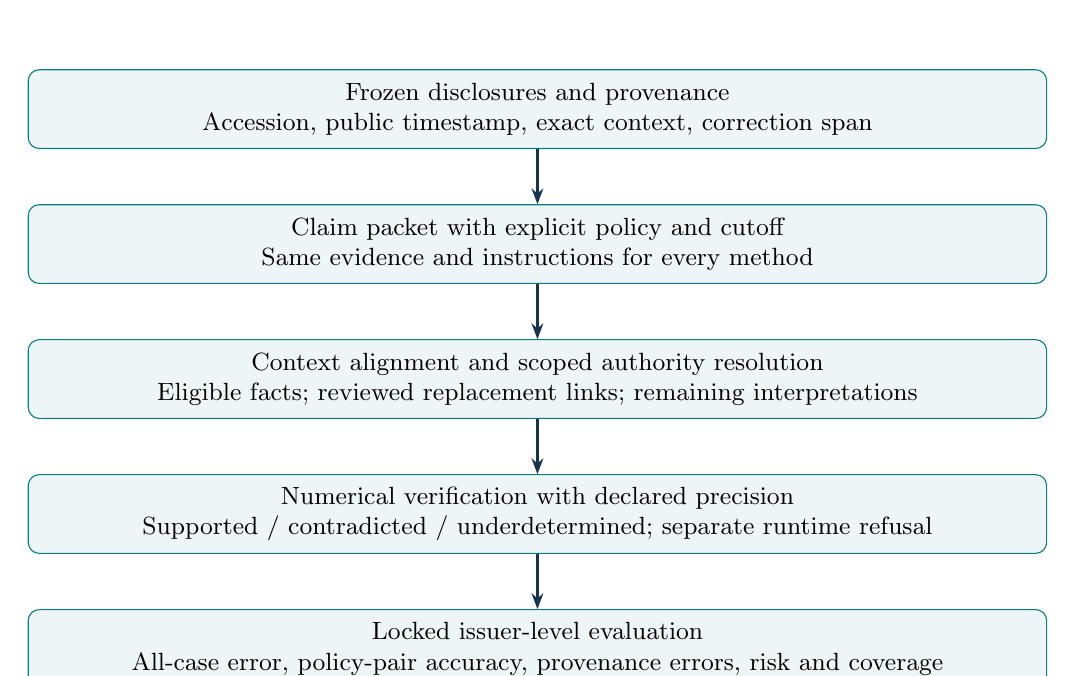
\begin{tikzpicture}[node distance=7mm,box/.style={draw=teal,fill=pale,rounded corners,align=center,text width=12.7cm,minimum height=10mm,font=\small},arr/.style={-{Stealth[length=2mm]},thick,draw=navy}]
\node[box](a){Frozen disclosures and provenance\\Accession, public timestamp, exact context, correction span};
\node[box,below=of a](b){Claim packet with explicit policy and cutoff\\Same evidence and instructions for every method};
\node[box,below=of b](c){Context alignment and scoped authority resolution\\Eligible facts; reviewed replacement links; remaining interpretations};
\node[box,below=of c](d){Numerical verification with declared precision\\Supported / contradicted / underdetermined; separate runtime refusal};
\node[box,below=of d](e){Locked issuer-level evaluation\\All-case error, policy-pair accuracy, provenance errors, risk and coverage};
\draw[arr](a)--(b);\draw[arr](b)--(c);\draw[arr](c)--(d);\draw[arr](d)--(e);
\end{tikzpicture}
\caption{Proposed study pipeline. Gold annotations are evaluation assets; their availability to a method depends on the track. No component has been implemented or benchmarked in this proposal.}
\end{figure}

\lead{Track A: controlled resolution.} All methods receive the same reviewed fact records, correction candidates, documentary spans, policy, and cutoff. This isolates interpretation and authority selection. It does not test whether a deployed system can extract the facts. Supplying gold edges only to the proposed resolver would be an invalid comparison; either all methods receive them or none do.

\lead{Track B: extraction plus resolution.} Every method receives the same raw disclosure packet and claim instructions. It must recover fact contexts and correction scope itself. A common frozen parser may be used by all structured methods; its misses count in all-case error. Human-corrected parsing is reported separately as an oracle diagnostic. The core laptop study uses deterministic extraction and reviewed rules; an optional small-model condition evaluates language interpretation without becoming a prerequisite for the benchmark.

\lead{Decision trace.} Each output records the selected accession(s), time eligibility, fact key, arithmetic expression, numerical interval, verdict, and uncertainty reason. An uncertain verdict can be correct, but its stated reason is evaluated against the annotation. A fluent explanation is not sufficient provenance.

\lead{Precommitment.} Freeze parser version, policy text, rounding rules, thresholds, baseline choice, and error taxonomy on the development set. Test evidence is opened only after the protocol is fixed. Changes made to repair a test-discovered defect create a clearly labeled subsequent evaluation; they do not replace the original result.

\pbreak
\section{Datasets, splits, leakage controls, and preprocessing}
\subsection{Primary source and acquisition contract}
\status{Proposed data.} Use public SEC filings from domestic US-GAAP issuers, initially 10-K and 10-Q reports with reporting periods in 2018--2025. Include 10-K/A or 10-Q/A only when the text establishes a relevant numerical change; also allow documented later comparative restatements. Freeze the evidence universe at 30 September 2026, before this proposal's literature review. These are acquisition boundaries, not claims that a suitable corpus already exists.

SEC submissions, Company Facts, and original filing archives provide discovery and provenance \cite{sec}. Company Facts cannot replace the original filing for dimensional or custom-concept evidence. Do not use the Frames endpoint to equate exact periods. Record accession, CIK, form, public acceptance timestamp when available, source URL, retrieval time, content hash, context identifier, unit, decimals, dimensions, and the precise correction/continuation span. Date-only availability records receive a conservative date-level rule; they cannot establish within-day order.

\lead{Sampling frame.} Start from a reproducible list of candidate issuers and amended filings, retaining every screening decision. Identify the correction family before writing claims. Log nonnumerical amendments, context changes, inaccessible files, and uncertain links. The retained dataset is a purposive challenge set, not a random sample of all financial claims. Its class balance and error rates must not be advertised as real-world prevalence.

\begin{table}[H]\caption{Conditional sample targets. The issuer, not the claim, is the primary inferential unit.}
\small\begin{tabularx}{\linewidth}{p{.22\linewidth}rrY}\toprule
Partition & Issuers & Claims & Role\\\midrule
Pilot, excluded & 5 & 30 & Check annotation instructions, acquisition, and timing. May be separate from a larger screening sample.\\
Development & 10 & 120 & Select/freeze extraction rules and operating thresholds.\\
Locked test & 40 & 480 & Primary evaluation; 12 claims per issuer.\\
Main total & 50 & 600 & Two correction families per issuer, six claim variants per family.\\\bottomrule
\end{tabularx}\end{table}

The target requires 100 reviewable families with authentic disclosures and researcher-authored claims. For each issuer, family 1 contributes three two-case pairs: original/latest policy switch, before/after cutoff switch, and unchanged-item invariance. Family 2 contributes specified/ambiguous-policy, precision-sensitive, and decisive negative-control pairs. Freeze exact templates after the excluded pilot. If a family cannot support the assigned pair, record the shortfall rather than force its label. These variants are not independent financial events.

\lead{Access and licensing.} The planned client would remain below two requests per second, below SEC's documented ten-per-second ceiling, with caching, backoff, and a truthful declared user agent \cite{secpolicy}. Public access does not imply unrestricted copyright over every embedded document. Release identifiers, short justified evidence excerpts, annotations, and acquisition instructions subject to rights review; do not promise blanket redistribution of entire filings. No credentials or paid data are required for the core design.

\pbreak
\subsection{Splits, annotation, and leakage controls}
\lead{Issuer-disjoint split.} Assign a whole issuer, all accessions, and all correction families to one partition before generating claims. Near-duplicate tables, subsidiary/parent overlaps, and shared merger histories are flagged; related entities are grouped when their evidence is substantially shared. Freeze the split manifest and its hash. Group stratification by sector and correction type is a balance aid, not evidence of independent sampling.

\lead{Time is a task input, not automatically a prospective split.} Each claim's cutoff limits its eligible evidence and annotations. The main experiment is retrospective with issuer holdout; it is not a deployment forecast. A later-period stress slice can test date sensitivity, but overlapping slices are not independent retraining windows. A pretrained language model may have seen public filings before this study. Evidence deletion and deliberately changed-context controls probe reliance on memorized facts; they do not prove absence of pretraining contamination \cite{kapoor}.

\lead{Annotation protocol.} Two reviewers independently mark each claim's exact context, eligible interpretations, correction links, numerical expression, precision, verdict, and evidence span. At least one reviewer needs financial-reporting competence. Hide system predictions from both. Preserve first-pass labels and disagreement reasons before adjudication. Report raw agreement and label-wise confusion; any chance-corrected coefficient is supplementary because class balance and structured partial agreement matter. Adjudicated labels are the benchmark's operational standard, not infallible truth.

\begin{table}[H]\caption{Leakage controls and the failure each prevents.}
\small\begin{tabularx}{\linewidth}{YY}\toprule
Control & Failure prevented / residual limitation\\\midrule
Whole-issuer and family split & Near-duplicate claim leakage; sector-level common shocks can remain.\\
Availability attached to facts and mappings & Future correction notes silently determining historical answers; date-only records limit precision.\\
Development-only rule/threshold selection & Test-driven tolerance, prompt, and parser tuning; test repairs require a new labeled round.\\
Shared packet and parsing track & Retrieval or gold-edge advantages mistaken for reasoning gains; controlled track remains an oracle setting.\\
Blinded independent annotation & Labels drifting toward system output; expert disagreement may still reflect real ambiguity.\\
Versioned source and model manifest & Unnoticed source/model changes; unavailable model snapshots are disclosed rather than reconstructed.\\\bottomrule
\end{tabularx}\end{table}

\lead{Missing and disputed evidence.} Keep genuinely unresolved cases as $\Ulabel$ when they satisfy the annotation contract. Exclude cases whose basic evidence authenticity or issuer identity cannot be established, with reasons recorded. A contradicted claim requires positive incompatible evidence; absence of a matching number is not enough. Scope-changing corrections may be retained as uncertainty controls, but cannot be mislabeled as exact same-key replacements.

\lead{No outcome-dependent filtering.} Test cases are not dropped because a baseline performs poorly, a proposed rule fails, or reviewers initially disagree. Report results both with all adjudicated cases and a preregistered high-confidence subset. The subset analysis is secondary and includes its selection rate.

\pbreak
\subsection{Preprocessing and audit of rejected datasets}
\lead{Financial evidence.} Preserve raw strings alongside canonical numeric values. Parentheses, dash glyphs, missing cells, percent signs, currency symbols, scaling, and duplicated labels have separate interpretations. A blank is not zero. Match exact start/end dates, instant versus duration, taxonomy version, consolidated versus segment scope, and currency before arithmetic. Do not combine currencies without an explicit exchange-rate fact and conversion date; the core benchmark excludes such conversions. Table totals with incompatible definitions are not forced to satisfy an identity.

\lead{Sensitive information.} The selected study concerns corporate disclosures, not individual borrowers. No protected attribute is needed for verification. Avoid extracting personal identifiers from incidental filing text. Sector, issuer size, reporting complexity, and document quality are audit strata; they are not automatically protected legal classes. Imbalanced representation across these strata limits external validity.

The original alternatives use different data. Their facts must still be audited even though they are not inputs to the selected experiment. The following corrections prevent an apparent merger from smuggling unsupported temporal or fairness claims into this proposal.

\begin{table}[H]\caption{Dataset audit for the rejected credit/fraud branches. These datasets are not required by the chosen study.}
\footnotesize\begin{tabularx}{\linewidth}{p{.16\linewidth}YY}\toprule
Dataset & Verified scope and unresolved facts & Required decision if that branch were revived\\\midrule
HELOC & An OpenML raw version has 10,459 rows; other versions differ \cite{heloc}. The exact 9,871 cleaned count and field-specific special-code dictionary were not tied to the same retrieved file. & Pin file/hash/version; establish meanings of $-9,-8,-7$ per field. Preserve missingness indicators; never treat them as continuous measurements or invent their semantics.\\
Taiwan credit & UCI documents 30,000 observations and 23 predictors \cite{taiwan}. Fields include PAY\_0 and PAY\_2 through PAY\_6; within-row history is not a longitudinal retraining panel. & Retain undocumented repayment-status codes as explicit categories pending a dictionary. Exclude SEX/MARRIAGE from prediction by design if reused; justify any audit access. Age handling needs context, not a universal monotonicity rule.\\
Bank Account Fraud suite & Synthetic variants with one million rows and eight months are documented \cite{baf}. Sensitive fields and temporal shifts are generator-dependent. & Evaluate full held-out months. Do not call synthetic results real bank deployment evidence. Income can be an audit covariate without being a legally protected class.\\\bottomrule
\end{tabularx}\end{table}

\lead{Subsampling correction, derived.} If all positives are kept and each negative is independently retained with probability $r\in(0,1]$, let $p$ be the population posterior and $p_s$ the sampled posterior. Bayes' rule gives $p_s=p/[p+r(1-p)]$, hence
\[
p=\frac{r p_s}{r p_s+1-p_s}.
\]
This requires class-conditional random sampling and a calibrated sampled posterior. Evaluating on a full test set does not itself repair sampled probabilities or thresholds. The selected challenge set likewise cannot estimate deployment prevalence: its deliberately selected claim mix is not corrected merely by reweighting without a defensible population sampling model.

\pbreak
\section{Experimental design}
\subsection{Baselines and information parity}
\begingroup\small
\begin{table}[H]\caption{Required core baselines and an optional language-model condition. All receive the same claim, policy, cutoff, and track-specific evidence.}
\small\begin{tabularx}{\linewidth}{p{.07\linewidth}>{\raggedright\arraybackslash}p{.24\linewidth}YY}\toprule
ID & Method & Capability / limitation & Role\\\midrule
B0 & Any-number match & Finds a matching number in the packet without context resolution. & Sanity control only; beating it establishes little.\\
B1 & Exact-context symbolic verifier & Matches entity, concept, unit, scope, and period; checks arithmetic. Conflicting versions remain unresolved. & Isolates benefit beyond ordinary context checks.\\
B2 & Unrestricted latest-fact rule & Selects the newest same-context fact, including disclosures after the requested cutoff. & Deliberately invalid temporal control, clearly labeled.\\
B3 & Cutoff-aware latest-fact rule & Uses eligible same-context facts; always selects the newest remaining value. & Tests simple chronology; no automatic deployment claim.\\
B4 & Policy-aware structured latest baseline & Honors a named original accession for as-filed claims; otherwise uses B3, with the same numerical checks and uncertainty rules as the resolver. & Primary strong baseline. It already receives and uses policy instructions.\\
B5 & Independent full policy-aware control & Implements the same admissible-interpretation contract from the written specification using a separately reviewed decision table. & Equivalence/control condition. A tie is expected to be plausible, not an algorithmic defeat to conceal.\\
P & Scoped-authority resolver & Uses documented, key-specific replacement links; preserves incomparable alternatives; propagates precision. & Proposed transparent reference method.\\
L & Policy-prompted small language model & Receives all instructions and evidence; outputs a structured verdict and provenance. & Optional empirical comparator, conditional on a runnable pinned model and budget.\\\bottomrule
\end{tabularx}\end{table}

\lead{Primary comparison.} P versus B4 is fixed in advance. B4 already handles original-as-filed claims. The discriminating cases concern scoped corrections, incomparable disclosures, mapping availability, and precision. If these are rare or P fails to extract them, H1 can fail.

\lead{Closest published systems.} Reuse faithful, licensed VeriFin/FinGround/AUDITFLOW releases where feasible \cite{verifin,finground,auditflow}; otherwise call these \emph{inspired baselines}, not reproductions. The core study cannot claim superiority over untested published systems. A policy-prompted LLM is required before claiming an advantage over LLM verification; if it cannot run, narrow the comparison.

\lead{Information parity.} All Track A methods receive reviewed edges. Track B uses shared raw packets. Report extraction cost and performance; human annotation must not masquerade as autonomous reasoning.
\endgroup

\pbreak
\subsection{Metrics and estimands}
Let $N$ be the number of evaluated claims, $y_i\in\{\Slabel,\Clabel,\Ulabel\}$ the gold label, and $\hat y_i\in\{\Slabel,\Clabel,\Ulabel,\Rlabel\}$ the output for claim $i$. Let $A_i=\ind\{\hat y_i\in\{\Slabel,\Clabel\}\}$ denote a decisive answer. The indicator $\ind\{B\}$ is one when statement $B$ holds and zero otherwise.
\[
\mathrm{Err}=\frac1N\sum_{i=1}^N\ind\{\hat y_i\ne y_i\},\qquad
\mathrm{Cov}=\frac1N\sum_{i=1}^N A_i.
\]
All operational refusals are errors in Err. A correct $\Ulabel$ prediction is not an error, but it does not count as decisive coverage. Define selective risk only when $\sum_i A_i>0$:
\[
\mathrm{Risk}=\frac{\sum_i A_i\ind\{\hat y_i\ne y_i\}}{\sum_i A_i}.
\]
At zero decisive coverage, risk is \emph{undefined}, not zero. Report counts, label-wise recall, macro-F1 with its explicit zero-denominator convention, and the full confusion matrix alongside these quantities. A majority-label system is a useful additional diagnostic.

\begin{table}[H]\caption{Secondary endpoints. Each denominator and failure type remains explicit.}
\small\begin{tabularx}{\linewidth}{p{.28\linewidth}Y}\toprule
Endpoint & Operational definition\\\midrule
False support & Fraction of gold $\Clabel$ predicted $\Slabel$; separately fraction of gold $\Ulabel$ predicted $\Slabel$. Report each denominator.\\
False contradiction & Fraction of gold $\Slabel$ predicted $\Clabel$. Decisive outputs on gold $\Ulabel$ are separately counted.\\
Policy-pair success & Fraction of annotated pairs with \emph{both} verdicts correct. Report expected-flip and invariant-control strata separately.\\
Time / authority errors & Fraction using an ineligible future disclosure; fraction using an unjustified replacement or wrong fact scope. Can overlap with numerical errors.\\
Provenance accuracy & Exact accession/context correctness and span sufficiency, judged blind to method. A correct label with wrong evidence is recorded as such.\\
Uncertainty quality & Precision/recall for gold $\Ulabel$, with runtime $\Rlabel$ separately counted; reasons compared with annotations.\\
Resource use & Wall time, peak memory, evidence volume, model/API cost where used, and manual correction minutes.\\\bottomrule
\end{tabularx}\end{table}

\lead{Issuer-level target.} Let $n_g$ be the number of claims for test issuer $g$, and $e_{mg}$ method $m$'s mean all-case error on those claims. With $G$ issuers, the primary effect is $\Delta=G^{-1}\sum_{g=1}^G(e_{B4,g}-e_{P,g})$. Positive $\Delta$ favors P. Report this equal-issuer average even if case counts become uneven. A pooled claim average is secondary; six variants of one event must not dominate the evidence.

\lead{Operating points.} Order optional rejection thresholds by a development-locked confidence/trace-quality rule with a fixed tie rule. Report the full attainable risk--coverage curve and the threshold chosen for development coverage 0.80. Test coverage may differ. Do not interpolate a deterministic method into an unattainable point and claim that it achieved it.

\pbreak
\subsection{Statistical testing and sample adequacy}
\lead{Independence assumption.} Test issuers are treated as approximately independent units for inference; claims, correction families, seeds, and repeated model calls within an issuer are not independent replicates. Shared sectors, accounting rules, and macroeconomic shocks can weaken this assumption. Report sector-block sensitivity and descriptive results when there are too few blocks. This is an inference about the constructed issuer population under stated assumptions, not all future filings \cite{demsar}.

Let $D_g=e_{B4,g}-e_{P,g}$. For the primary exact two-sided sign test, discard ties and let $n$ be the number of nonzero issuer differences and $W$ the number with $D_g>0$. Under the null $\Pr(D_g>0\mid D_g\ne0)=1/2$ and independence, $W\sim\mathrm{Binomial}(n,1/2)$. The test addresses consistency of direction across issuers, not directly equality of mean error. Report $\Delta$, its issuer-bootstrap 95\% interval, and the sign-test result as distinct summaries. Bootstrap intervals are approximate with 40 purposively selected clusters.

\lead{Multiplicity.} If H1--H3 receive formal tests, sort their valid two-sided $p$-values as $p_{(1)}\le p_{(2)}\le p_{(3)}$ and apply Holm thresholds $0.05/(4-j)$ at step $j\in\{1,2,3\}$ \cite{holm}. H2 uses the same sign procedure on issuer-level errors within the authority-sensitive stratum. H3 uses issuer-level selective-risk differences only if both methods have nonzero decisive answers for every issuer and overall achieved coverage lies within the preregistered 0.75--0.85 band. Otherwise H3 is descriptive and is assigned $p=1$ for the planned family, without changing the other thresholds. Report the coverage mismatch even when the condition is met.

\lead{Minimum units are not adequate power.} The smallest attainable two-sided exact sign-test $p$-value is $2/2^n$. For $M$ planned comparisons, even the most favorable data cannot cross the first Holm threshold unless
\[
n\ \ge\ \left\lceil\log_2\left(\frac{2M}{0.05}\right)\right\rceil.
\]
This gives six nonzero independent pairs for one comparison, seven for three, and nine for nine. These are algebraic feasibility minima, not recommended sample sizes. Ties reduce $n$. Signed-rank tests need additional distributional assumptions; replacing a sign test by Wilcoxon does not make overlapping windows independent.

\lead{Planning scenario.} If issuer differences had standard deviation 0.20, a normal mean-difference approximation for a 0.10 effect, two-sided 5\% level, and 80\% power gives $[(1.96+0.84)0.20/0.10]^2=31.36$, rounded to 32 issuers. This is a stated approximation for a mean test, \emph{not} a power guarantee for the sign test, Holm family, or clustered benchmark. The target is 40 test issuers. Pilot estimates may revise the target before test access; a revision and its assumptions are recorded. If fewer than 32 are feasible, label the study exploratory and emphasize intervals rather than significance.

For a sign-test power calculation, let $\theta$ be the assumed probability of a positive nonzero difference, $\alpha$ the nominal level, and $\mathcal R_{n,\alpha}$ its exact rejection set of positive-sign counts $w$. Power is $\sum_{w\in\mathcal R_{n,\alpha}}\binom nw\theta^w(1-\theta)^{n-w}$. No value is asserted without specifying $\theta$, ties, and the multiplicity threshold.

\pbreak
\subsection{Ablations, windows, and robustness analyses}
\begin{table}[H]\caption{One-factor ablations, with evidence and other rules held fixed.}
\small\begin{tabularx}{\linewidth}{p{.28\linewidth}YY}\toprule
Ablation & Question & Diagnostic, not automatic success\\\midrule
Remove cutoff filter & Does future evidence drive apparent accuracy? & Cutoff breaches and historical-pair failure.\\
Use document-wide replacement & Does amendment scope matter? & Errors on unchanged line items and scope changes.\\
Replace edges with latest timestamp & Do documented correction relations add value? & P versus B4, especially incomparable surviving facts.\\
Ignore dimensions / exact intervals & Are gains really basic context matching? & Scope and quarter-versus-year-to-date errors.\\
Ignore rounding intervals & Does point comparison create false confidence? & Errors concentrated near precision boundaries.\\
Force binary verdicts & Is underdetermination necessary? & Decisive errors on gold $\Ulabel$, alongside increased coverage.\\
Oracle parsing versus raw packet & How much error comes from extraction? & Gap between Tracks A and B, with equal information in each.\\\bottomrule
\end{tabularx}\end{table}

\lead{Temporal windows.} The selected study's primary independent units are issuers, so it does not require fictitious rolling windows. If a secondary temporal comparison uses independent nonoverlapping windows, it needs at least six nonzero windows for one exact two-sided test, seven for the planned three-test Holm family, and nine for nine tests merely to attain the respective threshold. Overlapping windows, repeated seeds, or four calendar quarters do not meet those conditions. The source BAF design offers only two full origins for its stated three-step horizon, which is insufficient for that inference; static HELOC/Taiwan resamples cannot repair it.

\lead{Distribution and construction checks.} Report performance separately for authentic correction types, researcher-authored false claims, neutral policy controls, ambiguous cases, and rounding-sensitive cases. Vary the proportion of $\Ulabel$ cases only as a labeled sensitivity analysis. Reweighting a challenge set does not identify the natural prevalence of misleading financial claims.

\lead{Reproducibility contract.} Publish the frozen protocol, data identifiers, permissible excerpts, split and annotation manifests, model/prompt/parser versions, full outputs, and documented deviations when the future study is run. All stochastic seeds are recorded, but seed variation is computational repeatability, not an increase in statistical sample size. This proposal itself supplies documents only and makes no claim that an executable experiment already exists.

\lead{Analysis boundaries.} Use one locked primary comparison, a small number of prespecified strata, and the ablations above. Avoid selecting the best significance result from numerous thresholds, windows, or error slices. Any additional discovered pattern is labeled exploratory and used to motivate a later study rather than silently replacing the primary hypothesis.

\pbreak
\section{Expected contributions and honest novelty claim}
\begin{decisionbox}
\lead{Defensible claim.} The study would provide an auditable evaluation of financial verification under explicit historical and correction-authority policies, using authentic disclosure relationships, paired claims, and equal-evidence baselines. It would test whether fact-scoped authority handling improves over strong simple rules. The review does not establish a new general verification algorithm or the first use of time, XBRL, arithmetic, provenance, or abstention in financial NLP.
\end{decisionbox}

\subsection{Contributions conditional on completing the study}
\lead{C1: an evaluation object.} A curated set of original/corrective disclosure families, paired policy-conditioned claims, source spans, and explicit uncertainty labels. Its value depends on authentic provenance and the absence of answer leakage. Merely changing dates in synthetic templates is not enough.

\lead{C2: a precise task contract.} A distinction between reporting period, public availability, authority policy, and acquisition time; fact-scoped replacement; conservative numerical precision; and separate gold uncertainty versus operational refusal. These formalize the evaluation and expose failure cases. They are not advertised as a novel theorem beyond the elementary propositions in Section 7.

\lead{C3: evidence about minimal sufficiency.} A comparison of exact-context checks, cutoff-aware latest selection, scoped authority resolution, and an independent full-policy control. A policy-aware prompt may be sufficient. A transparent reference resolver may be useful without being superior to every modern verifier.

\lead{C4: a reusable error analysis.} Distinguish extraction, context, time eligibility, replacement scope, arithmetic, and uncertainty errors. Categories may overlap; a label and a mechanism are not interchangeable. The output is a diagnostic account of failure, not a single leaderboard number stripped of coverage and provenance.

\subsection{What would undermine the claim}
An existing released benchmark with equivalent authentic authority-switch cases would reduce C1 to replication or extension. FinGround's explicit restatement handling already narrows any broad “first period-aware financial verifier” claim \cite{finground}; VeriFin and AUDITFLOW narrow claims about symbolic checking \cite{verifin,auditflow}. If B4 or the independent policy-aware control matches P, C3 becomes evidence that simple specification suffices. If only gold-parsed Track A succeeds, the contribution is a controlled benchmark, not a working autonomous filing auditor.

\lead{Venue fit.} The likely manuscript should be framed for financial NLP evaluation, AI in finance, or a benchmark/resource track. It needs credible annotation, accessible evidence, and informative strong baselines. A general machine-learning theory venue would be a poor fit for the present elementary propositions. No venue acceptance or impact level is promised.

\lead{Attribution.} P2 supplies the selected problem family; P1 supplies temporal leakage discipline and the requirement to test simple alternatives; P3 supplies caution about mathematical guarantees, data semantics, and inadequate independent samples. The final study does not inherit the sources' unexecuted performance expectations.

\pbreak
\section{Limitations and threats to validity}
\begin{table}[H]\caption{Threats, their implications, and what the study can realistically check.}
\small\begin{tabularx}{\linewidth}{p{.15\linewidth}YY}\toprule
Validity & Threat and implication & Control and remaining limit\\\midrule
Internal & Gold correction links could favor P; reviewers might use future evidence for historical labels. & Equal inputs within track; timestamp annotation provenance; blinded double review. Human judgment remains fallible.\\
Internal & Parser errors or unequal retrieval can mimic reasoning gains. & Shared packet, controlled parsed track, explicit oracle diagnostic. Controlled performance does not establish deployment capability.\\
External & US-GAAP, SEC, and purposive correction cases omit other jurisdictions, languages, and ordinary filings. & Describe the sampling frame and rejected cases. No global financial-verification prevalence claim.\\
External & Small issuers or complex filings may be underrepresented because they are harder to annotate. & Report size/sector/document-quality strata and screening attrition. Do not infer fairness from balanced counts alone.\\
Construct & Researcher-authored claims may be unnatural; authority policies may be more explicit than real user queries. & Separate natural evidence from constructed language; include unspecified-policy cases. This remains a benchmark of a defined contract.\\
Construct & Intervals may be conservative; accounting concepts may not be equivalent despite similar labels. & Reviewed mappings and precision notes; uncertainty instead of forced equality. More $\Ulabel$ outputs may reflect a cautious contract.\\
Statistical & Many claims but few issuers; correlated sectors; ties and class imbalance. & Issuer-level estimates and inference; report denominators and intervals. Forty issuers is a target, not a universal adequacy theorem.\\
Statistical & Threshold selection and multiple error slices invite optimism. & Development-only tuning, one primary contrast, Holm family where valid, exploratory labeling. Small secondary strata remain descriptive.\\\bottomrule
\end{tabularx}\end{table}

\lead{Literature coverage.} Bibliographic identity is verified more broadly than full-text methods. Some 2026 papers are preprints, and method/version changes can alter the comparison. The search identified strong close work, but could miss a recently released equivalent dataset. The proposal therefore makes a dated, bounded novelty claim and a precollection update commitment.

\lead{Annotation authority.} SEC acceptance establishes that a submission was received and made available; it does not certify the issuer's economic truth. A supported verdict means supported under the stated disclosure contract. The study does not audit accounting fraud, certify financial statements, or replace professional financial review.

\lead{Operational limitations.} A laptop can plausibly run the structured core, but no wall-time measurement has yet been made. Extraction quality, amendment yield, and qualified reviewer availability are the critical unknowns. Optional language-model results require a pinned model and declared resource use; they cannot be silently replaced by a stronger paid model after seeing the test labels.

\pbreak
\section{Risks, mitigation, and a negative-result plan}
\begin{table}[H]\caption{Research risks and predeclared responses.}
\small\begin{tabularx}{\linewidth}{p{.27\linewidth}YY}\toprule
Risk & Trigger / gate & Response\\\midrule
Insufficient authentic numerical corrections & Week 2: fewer than 20 screened eligible families across 10 issuers, or fewer than 30 usable pilot claims. & Narrow the correction type or publish a feasibility pilot; do not manufacture “natural” cases.\\
Ambiguous authority labels & Reviewers cannot justify a replacement from eligible text. & Keep as $\Ulabel$ if within contract; otherwise exclude with a recorded reason. Never force a decisive label to balance classes.\\
Closest work duplicates the task & Supplement/code review reveals equivalent policies and cases. & Reframe as replication, comparative audit, or targeted extension; revise novelty language before data collection.\\
No advantage over B4/B5 & Error interval includes zero or practical difference is negligible. & Publish benchmark and sufficiency boundary; do not search retrospectively for a favorable primary metric.\\
Only oracle parsing succeeds & Track B loses the controlled-track gain. & Attribute the bottleneck to extraction; do not claim autonomous authority reasoning.\\
Annotation time exceeds budget & Pilot timing projects more than available researcher/reviewer hours. & Reduce scope transparently and downgrade inference; preserve independent review for retained cases.\\
Access or redistribution constraints & SEC throttling, inaccessible records, or rights uncertainty. & Cache/back off; use identifiers and permitted excerpts; document attrition and release limits.\\\bottomrule
\end{tabularx}\end{table}

\lead{If H1 fails.} The manuscript becomes “When explicit policy and simple metadata suffice for financial claim verification.” Report the original primary endpoint, interval, and error distribution. If the independent policy-aware control ties P, explain that the benchmark isolates a specification problem rather than supporting architectural novelty.

\lead{If H2 fails.} If gains vanish under equal parsed facts, document retrieval or extraction as the true source. If policy-sensitive pairs are solved but invariance controls degrade, report the tradeoff rather than celebrating only flips. Preserve every preregistered stratum.

\lead{If H3 fails.} Publish risk--coverage curves, unattainable operating points, and the cost of uncertainty. All-refusal behavior is explicitly penalized in all-case error and has undefined selective risk. A conservative specification can be correct yet operationally unhelpful; the paper must say so.

\lead{If H5 fails.} A small manually reviewed case study can still establish an annotation protocol and a transparent acquisition limitation. It cannot support a broad benchmark ranking. Include screening denominators, attrition reasons, and the observed reviewer workload once measured. A documented inability to acquire reliable labels is more informative than invented scale.

\pbreak
\section{Feasibility: compute, access, and milestones}
\status{Planning assumptions.} One researcher contributes up to 320 hours over eight research weeks, followed by two writing/release weeks. A second reviewer with suitable financial-reporting competence contributes approximately 40--50 hours. That reviewer is a resource requirement, not an already secured collaborator. The core uses public filings, deterministic parsing/lookup, and small tables; it requires no model training, paid API, or GPU.

\begin{table}[H]\caption{Ten-week proposed schedule with concrete gates and outputs.}
\small\begin{tabularx}{\linewidth}{p{.10\linewidth}YY}\toprule
Week & Work and milestone & Decision / deliverable\\\midrule
1 & Update closest-work review; freeze schema, policy text, sampling frame, and rights plan. & Written protocol and amended novelty statement.\\
2 & Screen at least 20 eligible families across 10 issuers; double-annotate 30 pilot claims from five excluded issuers. & Acquisition/annotation gate; stop or narrow if unsupported.\\
3--4 & Acquire and annotate main evidence; finalize issuer split; adjudicate development cases. & Provenance manifest and frozen development package.\\
5 & Complete locked-test annotation; review shared evidence and parser contracts. & Test labels sealed; annotation report.\\
6 & Future implementation/runs of required baselines and resolver, after this proposal stage. & Frozen methods and full raw outputs.\\
7 & Locked evaluation, prespecified ablations, issuer-level uncertainty. & Primary/secondary result tables, including failures.\\
8 & Error review and resource accounting; no retrospective primary-endpoint substitution. & Audited analysis and release decision.\\
9--10 & Write manuscript; prepare permissible benchmark materials and documentation. & Submission-ready draft conditional on study quality.\\\bottomrule
\end{tabularx}\end{table}

\lead{Human effort estimate.} At an assumed six minutes per claim, first annotation of 600 claims costs 60 hours. At three minutes per claim, independent review costs 30 hours, plus an assumed 10--20 hours of adjudication. Screening/acquisition is budgeted at 60 researcher hours. These are planning scenarios to be replaced by pilot measurements, not evidence that financial review is routinely this fast. Complex families may require considerably more time.

\lead{Compute envelope.} Plan for a laptop with 16 GB RAM, four or more CPU cores, and up to 20 GB temporary storage; these are resource assumptions, not benchmarked requirements. Cache original evidence and structured records, process filings incrementally, and cap the corpus before exceeding available disk. The optional local model is admitted only after a development-only memory/runtime check. An optional external API budget is capped at US\$100 and is unnecessary for the core; any use changes the reported cost and data-handling record.

\lead{Feasibility judgment.} Computational cost is unlikely to be the dominant constraint for the structured core, but this remains a hypothesis until measured. Authentic correction yield, accounting interpretation, and independent annotation are the hard dependencies. If a second reviewer is unavailable, the final product must be labeled a single-annotator pilot, with correspondingly narrower claims.

\pbreak
\section{Ethics, fairness, and regulatory considerations}
\lead{Research scope.} This is a proposed study of public corporate disclosures. It does not decide credit eligibility, recommend trades, or supply borrower recourse. A verdict is evidence-relative and can be wrong. Release examples with their provenance, authority policy, and limitations so that a decontextualized “false” label is not mistaken for an allegation of corporate misconduct.

\lead{ECOA / Regulation B.} The source documents' four-feature compliance rationale is rejected. Regulation B requires specific principal reasons in its applicable adverse-action framework, or prescribed notice of the right to receive them; its official interpretation does not fix the number. Sex and marital status, age, income source, and related variables have specific restrictions and exceptions in 12 CFR 1002.6. A broad claim that every use of age is prohibited is inaccurate. A public Taiwan dataset is not automatically governed by US law \cite{regb}. These provisions do not require this corporate-verification method.

\lead{FCRA.} Relevant adverse-action notices and score disclosures depend on the statutory trigger. The score-factor limit is generally four, or five if inquiries are a key factor; it is distinct from a creditor's principal reasons. Neither a feature-importance ranking nor an algorithmic action plan automatically satisfies these duties \cite{fcra,regb,barocas}. The final proposal does not claim legal compliance from explanation length.

\lead{EU AI Act.} Annex III 5(b) identifies natural-person creditworthiness/credit-score systems as a high-risk use case, except systems used to detect financial fraud. The exception is not an exemption from the entire Act. Article 86 concerns explanations of certain consequential decisions based on covered high-risk outputs; it is not a general right to a successful counterfactual action. Article 2's research exclusions have conditions and do not justify treating every real-world research deployment as exempt \cite{aiact}.

\begin{decisionbox}
\lead{Dated legal-source conflict.} On 23 October 2026, the retrieved Commission AI Act Service Desk stated that its text reflected a consolidated version of 27 July 2026, and displayed 2 December 2027 for the relevant Annex III high-risk provisions in Article 113. Its linked FAQ retained proposal language and older dates. The original EUR-Lex URLs returned no usable text in this audit. The substantive clauses above were checked, but a universal current enforcement date is \emph{not certified}. The source claim of blanket August 2026 enforcement is therefore not adopted.
\end{decisionbox}

\lead{Fairness and representation.} Report performance by sector, issuer size, document complexity, and correction type where denominators permit. These are coverage diagnostics, not a substitute for a protected-class fairness analysis in a future credit-decision application. Do not infer equal treatment of borrowers from good financial-document accuracy. Avoid collecting personal identifiers, honor source rights, and document any model/API transfer of evidence.

\lead{Release and accountability.} Use an institutional ethics review if locally required for the eventual study; no such approval is represented as already obtained. Provide a correction process for annotation disputes, preserve source versions, and explain that public filings and automated interpretations can both contain errors. The research output supports inspection, not regulatory certification.

\pbreak
\refstepcounter{section}
\addcontentsline{toc}{section}{15. References}
\renewcommand{\refname}{15. References}
\begingroup\small
\begin{thebibliography}{99}
\setlength{\itemsep}{4pt}
\bibitem{sec} U.S. Securities and Exchange Commission. 2024. \emph{EDGAR Application Programming Interfaces (APIs)}. Page dated 6 June. \href{https://www.sec.gov/search-filings/edgar-application-programming-interfaces}{Official documentation}. Verified online; accessed 23 October 2026.
\bibitem{secpolicy} U.S. Securities and Exchange Commission. n.d. \emph{Developer Resources}. \href{https://www.sec.gov/about/developer-resources}{Official access policy}. Verified online; accessed 23 October 2026.
\bibitem{regb} Consumer Financial Protection Bureau. Current online text. \emph{Regulation B}, 12 CFR §§1002.6, 1002.9 and Supplement I. \href{https://www.consumerfinance.gov/rules-policy/regulations/1002/6/}{§6}; \href{https://www.consumerfinance.gov/rules-policy/regulations/1002/9/}{§9 and official interpretation}. Verified online; accessed 23 October 2026.
\bibitem{fcra} United States Congress. 2023 compilation. \emph{Fair Credit Reporting Act}, 15 USC §§1681g(f), 1681m(a). \href{https://www.ftc.gov/system/files/ftc_gov/pdf/fcra-may2023-508.pdf}{FTC statutory compilation}. Verified online; accessed 23 October 2026.
\bibitem{aiact} European Parliament and Council. 2024. \emph{Regulation (EU) 2024/1689}. OJ L, 12 July 2024. Commission Service Desk: \href{https://ai-act-service-desk.ec.europa.eu/en/ai-act/annex-3}{Annex III}, Articles \href{https://ai-act-service-desk.ec.europa.eu/en/ai-act/article-2}{2}, \href{https://ai-act-service-desk.ec.europa.eu/en/ai-act/article-86}{86}, \href{https://ai-act-service-desk.ec.europa.eu/en/ai-act/article-113}{113}. Retrieved text displays a 27 July 2026 consolidated version. Clauses verified online; transition-date reconciliation unresolved. Accessed 23 October 2026.
\bibitem{jensen} Christian S. Jensen and Richard T. Snodgrass. 1999. Temporal data management. \emph{IEEE Transactions on Knowledge and Data Engineering} 11(1):36--44. \href{https://doi.org/10.1109/69.755613}{doi:10.1109/69.755613}. Verified online; accessed 23 October 2026.
\bibitem{mori} Marco Mori, Paolo Papotti, Luigi Bellomarini, and Oliver Giudice. 2022. Neural Machine Translation for Fact-checking Temporal Claims. \emph{FEVER}, 78--82. \href{https://aclanthology.org/2022.fever-1.8/}{doi:10.18653/v1/2022.fever-1.8}. Verified online; accessed 23 October 2026.
\bibitem{chronofact} Anab Maulana Barik, Wynne Hsu, and Mong Li Lee. 2025. ChronoFact: Timeline-based Temporal Fact Verification. \emph{IJCAI}, 8031--8039. \href{https://www.ijcai.org/proceedings/2025/893}{doi:10.24963/ijcai.2025/893}. Verified online; accessed 23 October 2026.
\bibitem{ambifc} Max Glockner, Ieva Staliūnaitė, James Thorne, Gisela Vallejo, Andreas Vlachos, and Iryna Gurevych. 2024. AmbiFC: Fact-Checking Ambiguous Claims with Evidence. \emph{Transactions of the ACL} 12:1--18. \href{https://aclanthology.org/2024.tacl-1.1/}{doi:10.1162/tacl\_a\_00629}. Verified online; accessed 23 October 2026.
\bibitem{verifin} Bethel Hall, Sachi Shome, and William Eiers. 2026. VeriFin: A Neurosymbolic Framework for Verifying LLM-Generated Financial Claims. \href{https://arxiv.org/abs/2608.10213}{arXiv:2608.10213}, v2 inspected. Verified online, preprint; accessed 23 October 2026.

\pbreak
\bibitem{finground} Dongxin Guo, Jikun Wu, and Siu Ming Yiu. 2026. FinGround: Detecting and Grounding Financial Hallucinations via Atomic Claim Verification. \href{https://arxiv.org/abs/2604.23588}{arXiv:2604.23588}, v1 inspected. Verified online as preprint; source's later venue claim not independently established. Accessed 23 October 2026.
\bibitem{findver} Yilun Zhao, Yitao Long, Yuru Jiang, Chengye Wang, Weiyuan Chen, Hongjun Liu, Yiming Zhang, Xiangru Tang, Chen Zhao, and Arman Cohan. 2024. FinDVer: Explainable Claim Verification over Long and Hybrid-Content Financial Documents. \emph{EMNLP}, 14739--14752. \href{https://aclanthology.org/2024.emnlp-main.818/}{doi:10.18653/v1/2024.emnlp-main.818}. Verified online with unresolved PDF/landing metadata conflict; author names/order follow inspected PDF. Accessed 23 October 2026.
\bibitem{finverbench} Silu Panda. 2026. FinVerBench: Benchmark Validity and Calibration in Large Language Model Financial Statement Verification. \href{https://arxiv.org/abs/2605.29586}{arXiv:2605.29586}, v1 inspected. Verified online, preprint; accessed 23 October 2026.
\bibitem{auditflow} Yan Wang, Xuguang Ai, Jaisal Patel, Xueqing Peng, Fengran Mo, Yupeng Cao, Haohang Li, Mingyu Cao, Lingfei Qian, and Víctor Gutiérrez-Basulto. 2026. AUDITFLOW: Executable Symbolic Environments for Structured Financial Reporting Verification. \href{https://arxiv.org/abs/2606.03031}{arXiv:2606.03031}, v2 inspected. Verified online, preprint; accessed 23 October 2026.
\bibitem{faith} Mengao Zhang, Jiayu Fu, Tanya Warrier, Yuwen Wang, Tianhui Tan, and Ke-wei Huang. 2025. FAITH: A Framework for Assessing Intrinsic Tabular Hallucinations in Finance. \emph{ICAIF}, 159--167. \href{https://doi.org/10.1145/3768292.3770433}{doi:10.1145/3768292.3770433}. Metadata verified online; accessed 23 October 2026.
\bibitem{finqa} Zhiyu Chen, Wenhu Chen, Charese Smiley, Sameena Shah, Iana Borova, Dylan Langdon, Reema Moussa, Matt Beane, Ting-Hao Huang, Bryan Routledge, and William Yang Wang. 2021. FinQA: A Dataset of Numerical Reasoning over Financial Data. \emph{EMNLP}, 3697--3711. \href{https://aclanthology.org/2021.emnlp-main.300/}{doi:10.18653/v1/2021.emnlp-main.300}. Verified online; accessed 23 October 2026.
\bibitem{tatqa} Fengbin Zhu, Wenqiang Lei, Youcheng Huang, Chao Wang, Shuo Zhang, Jiancheng Lv, Fuli Feng, and Tat-Seng Chua. 2021. TAT-QA: A Question Answering Benchmark on a Hybrid of Tabular and Textual Content in Finance. \emph{ACL-IJCNLP}, 3277--3287. \href{https://aclanthology.org/2021.acl-long.254/}{doi:10.18653/v1/2021.acl-long.254}. Verified online; accessed 23 October 2026.
\bibitem{convfinqa} Zhiyu Chen, Shiyang Li, Charese Smiley, Zhiqiang Ma, Sameena Shah, and William Yang Wang. 2022. ConvFinQA: Exploring the Chain of Numerical Reasoning in Conversational Finance Question Answering. \emph{EMNLP}, 6279--6292. \href{https://aclanthology.org/2022.emnlp-main.421/}{doi:10.18653/v1/2022.emnlp-main.421}. Verified online; accessed 23 October 2026.
\bibitem{multihiertt} Yilun Zhao, Yunxiang Li, Chenying Li, and Rui Zhang. 2022. MultiHiertt: Numerical Reasoning over Multi Hierarchical Tabular and Textual Data. \emph{ACL}, 6588--6600. \href{https://aclanthology.org/2022.acl-long.454/}{doi:10.18653/v1/2022.acl-long.454}. Verified online; accessed 23 October 2026.
\bibitem{docfinqa} Varshini Reddy, Rik Koncel-Kedziorski, Viet Dac Lai, Michael Krumdick, Charles Lovering, and Chris Tanner. 2024. DocFinQA: A Long-Context Financial Reasoning Dataset. \emph{ACL short papers}, 445--458. \href{https://aclanthology.org/2024.acl-short.42/}{doi:10.18653/v1/2024.acl-short.42}. Verified online; accessed 23 October 2026.

\pbreak
\bibitem{financereasoning} Zichen Tang, Haihong E, Ziyan Ma, Haoyang He, Jiacheng Liu, Zhongjun Yang, Zihua Rong, Rongjin Li, Kun Ji, Qing Huang, Xinyang Hu, Yang Liu, and Qianhe Zheng. 2025. FinanceReasoning: Benchmarking Financial Numerical Reasoning More Credible, Comprehensive and Challenging. \emph{ACL}, 15721--15749. \href{https://aclanthology.org/2025.acl-long.766/}{doi:10.18653/v1/2025.acl-long.766}. Verified online with name conflict: export has Ziyan Ma; stored HTML has Tzu-Yen Ma. Accessed 23 October 2026.
\bibitem{t2ragbench} Jan Strich, Enes Kutay Isgorur, Maximilian Trescher, Chris Biemann, and Martin Semmann. 2026. T²-RAGBench: Text-and-Table Benchmark for Evaluating Retrieval-Augmented Generation. \emph{EACL}, 165--191. \href{https://aclanthology.org/2026.eacl-long.8/}{doi:10.18653/v1/2026.eacl-long.8}. Verified online; accessed 23 October 2026.
\bibitem{finmragbench} Shouqing Yang, Qi Zhang, Yuhang Yang, Ruikang Xu, Yuwei Hou, Zhulin Jia, Lirong Gao, Haobo Wang, Jinglei Chen, Jiexiang Wang, Sheng Guo, Bo Zheng, and Gang Chen. 2026. FinMRAGBench: A Realistic and Complex Benchmark for Multi-Modal RAG in Financial Document Analysis. \emph{Findings of ACL}, 3822--3867. \href{https://aclanthology.org/2026.findings-acl.187/}{doi:10.18653/v1/2026.findings-acl.187}. Verified online; accessed 23 October 2026.
\bibitem{financebench} Pranab Islam, Anand Kannappan, Douwe Kiela, Rebecca Qian, Nino Scherrer, and Bertie Vidgen. 2023. FinanceBench: A New Benchmark for Financial Question Answering. \href{https://arxiv.org/abs/2311.11944}{arXiv:2311.11944}. Verified online; author repository and dataset card also inspected. Accessed 23 October 2026.
\bibitem{ragtruth} Cheng Niu, Yuanhao Wu, Juno Zhu, Siliang Xu, KaShun Shum, Randy Zhong, Juntong Song, and Tong Zhang. 2024. RAGTruth: A Hallucination Corpus for Developing Trustworthy Retrieval-Augmented Language Models. \emph{ACL}, 10862--10878. \href{https://aclanthology.org/2024.acl-long.585/}{doi:10.18653/v1/2024.acl-long.585}. Verified online; accessed 23 October 2026.
\bibitem{factscore} Sewon Min, Kalpesh Krishna, Xinxi Lyu, Mike Lewis, Wen-tau Yih, Pang Koh, Mohit Iyyer, Luke Zettlemoyer, and Hannaneh Hajishirzi. 2023. FActScore: Fine-grained Atomic Evaluation of Factual Precision in Long Form Text Generation. \emph{EMNLP}, 12076--12100. \href{https://aclanthology.org/2023.emnlp-main.741/}{doi:10.18653/v1/2023.emnlp-main.741}. Verified online; accessed 23 October 2026.
\bibitem{selective} Yonatan Geifman and Ran El-Yaniv. 2017. Selective Classification for Deep Neural Networks. \emph{NeurIPS} 30; \href{https://arxiv.org/abs/1705.08500}{arXiv:1705.08500}. Preprint identity verified online; accessed 23 October 2026.
\bibitem{kapoor} Sayash Kapoor and Arvind Narayanan. 2023. Leakage and the reproducibility crisis in machine-learning-based science. \emph{Patterns} 4(9):100804. \href{https://doi.org/10.1016/j.patter.2023.100804}{doi:10.1016/j.patter.2023.100804}. Verified online; accessed 23 October 2026.
\bibitem{demsar} Janez Demšar. 2006. Statistical Comparisons of Classifiers over Multiple Data Sets. \emph{JMLR} 7:1--30. \href{https://www.jmlr.org/papers/v7/demsar06a.html}{Publisher record}. Verified online; accessed 23 October 2026.
\bibitem{holm} Sture Holm. 1979. A Simple Sequentially Rejective Multiple Test Procedure. \emph{Scandinavian Journal of Statistics} 6(2):65--70. \href{https://www.jstor.org/stable/4615733}{JSTOR stable 4615733}. Known standard reference; complete online record not recovered on 23 October 2026.

\pbreak
\bibitem{baf} Sérgio Jesus, José Pombal, Duarte Alves, André Cruz, Pedro Saleiro, Rita P. Ribeiro, João Gama, and Pedro Bizarro. 2022. Turning the Tables: Biased, Imbalanced, Dynamic Tabular Datasets for ML Evaluation. \emph{NeurIPS Datasets and Benchmarks}; \href{https://arxiv.org/abs/2211.13358}{arXiv:2211.13358}. Verified online, including official datasheet; accessed 23 October 2026.
\bibitem{dal2018} Andrea Dal Pozzolo, Giacomo Boracchi, Olivier Caelen, Cesare Alippi, and Gianluca Bontempi. 2018. Credit Card Fraud Detection: A Realistic Modeling and a Novel Learning Strategy. \emph{IEEE TNNLS} 29(8):3784--3797. \href{https://doi.org/10.1109/TNNLS.2017.2736643}{doi:10.1109/TNNLS.2017.2736643}. Verified online; accessed 23 October 2026.
\bibitem{bergmeir} Christoph Bergmeir, Rob J. Hyndman, and Bonsoo Koo. 2018. A note on the validity of cross-validation for evaluating autoregressive time series prediction. \emph{Computational Statistics \& Data Analysis} 120:70--83. \href{https://doi.org/10.1016/j.csda.2017.11.003}{doi:10.1016/j.csda.2017.11.003}. Verified online; accessed 23 October 2026.
\bibitem{topk} Tongchen Zhang, Zhen Zhang, Moxuan Zheng, Wenxi Sun, Xiao Han, Yao Xiao, and Junyi Yao. 2026. Cost-Sensitive Top-K Review for Capacity-Constrained Fraud Screening. \emph{IEEE Access} 14:152441--152457. \href{https://doi.org/10.1109/ACCESS.2026.3735481}{doi:10.1109/ACCESS.2026.3735481}. Metadata verified online; accessed 23 October 2026.
\bibitem{zuberi} Nikosi Zuberi, Md Mostafizur Rahman, Saeed Ur Rashid, Md. Naimul Ahsan, MD. Soebur Rahman, and Md Harun Or Rashid Mollah. 2026. A robust machine learning framework for detecting temporal drift in financial fraud prevention. \emph{Scientific Reports} 16; article 27776 is source-stated. \href{https://doi.org/10.1038/s41598-026-58285-5}{doi:10.1038/s41598-026-58285-5}. DOI/title/authors verified online; accessed 23 October 2026.
\bibitem{groupshapley} Martin Jullum, Annabelle Redelmeier, and Kjersti Aas. 2021. groupShapley: Efficient prediction explanation with Shapley values for feature groups. \href{https://arxiv.org/abs/2106.12228}{arXiv:2106.12228}. Verified online; accessed 23 October 2026.
\bibitem{rrf} Gordon V. Cormack, Charles L. A. Clarke, and Stefan Buettcher. 2009. Reciprocal rank fusion outperforms condorcet and individual rank learning methods. \emph{SIGIR}, 758--759. \href{https://doi.org/10.1145/1571941.1572114}{doi:10.1145/1571941.1572114}. Verified online; accessed 23 October 2026.
\bibitem{stow} May Stow. 2026. Quantifying Explanation Disagreement Between SHAP and LIME Across Tabular Classification Models. \emph{IJCSE} 14(1):13--21. \href{https://doi.org/10.26438/ijcse.v14i1.7255}{doi:10.26438/ijcse.v14i1.7255}. Publisher and metadata verified online; accessed 23 October 2026.
\bibitem{biomark} Mehmet Ali Balikci, Cyrille Mesue Njume, and Ali Cakmak. 2026. BioMark: biomarker analysis tool. \emph{BMC Bioinformatics} 27:42. \href{https://doi.org/10.1186/s12859-025-06346-3}{doi:10.1186/s12859-025-06346-3}. Publisher full text verified online; accessed 23 October 2026.
\bibitem{shapmcnemar} Passawish Gonlachanvit, Angsumalin Senjuntichai, and Teerapong Senjuntichai. 2026. SHAP-McNemar stepwise feature selection for machine learning in credit risk modeling. \emph{Machine Learning with Applications} 25:100977. \href{https://doi.org/10.1016/j.mlwa.2026.100977}{doi:10.1016/j.mlwa.2026.100977}. Metadata verified online; publisher full text blocked. Accessed 23 October 2026.

\pbreak
\bibitem{dutta} Sanghamitra Dutta, Jason Long, Saumitra Mishra, Cecilia Tilli, and Daniele Magazzeni. 2022. Robust Counterfactual Explanations for Tree-Based Ensembles. \emph{ICML, PMLR} 162:5742--5756. \href{https://proceedings.mlr.press/v162/dutta22a.html}{Publisher record}. Verified online; accessed 23 October 2026.
\bibitem{pawelczyk} Martin Pawelczyk, Teresa Datta, Johannes van den Heuvel, Gjergji Kasneci, and Himabindu Lakkaraju. 2023. Probabilistically Robust Recourse: Navigating the Trade-offs between Costs and Robustness in Algorithmic Recourse. \emph{ICLR}; \href{https://arxiv.org/abs/2203.06768}{arXiv:2203.06768}, first posted 2022. Preprint identity verified online; accessed 23 October 2026.
\bibitem{jabbari} Shahin Jabbari. 2026. Algorithmic Recourse Under Competition. \href{https://arxiv.org/abs/2609.39877}{arXiv:2609.39877}, first posted 30 September 2026. Sole listed author; verified online. Accessed 23 October 2026.
\bibitem{maalej} Aicha Maalej, Cecilia Sönströd, and Ulf Johansson. 2025. Counterfactual Explanations for Conformal Prediction Sets. \emph{COPA, PMLR} 266:405--424. \href{https://proceedings.mlr.press/v266/maalej25a.html}{Publisher record}. Verified online; accessed 23 October 2026.
\bibitem{barocas} Solon Barocas, Andrew D. Selbst, and Manish Raghavan. 2020. The hidden assumptions behind counterfactual explanations and principal reasons. \emph{FAT*}, 80--89. \href{https://doi.org/10.1145/3351095.3372830}{doi:10.1145/3351095.3372830}. Verified online; accessed 23 October 2026.
\bibitem{karimi} Amir-Hossein Karimi, Bernhard Schölkopf, and Isabel Valera. 2021. Algorithmic Recourse: from Counterfactual Explanations to Interventions. \emph{FAccT}, 353--362. \href{https://doi.org/10.1145/3442188.3445899}{doi:10.1145/3442188.3445899}. Verified online; DOI record uses the shortened main title. Accessed 23 October 2026.
\bibitem{heloc} FICO challenge data, version-specific OpenML repackaging. n.d. \emph{HELOC dataset metadata}. \href{https://www.openml.org/api/v1/json/data/46932}{OpenML 46932}; also 45023 and 45026. Verified online for version-specific counts; cleaned 9,871-row count and exact special-code dictionary unresolved. Accessed 23 October 2026.
\bibitem{taiwan} I-Cheng Yeh. 2009 deposit. \emph{Default of Credit Card Clients}. UCI dataset 350. \href{https://archive.ics.uci.edu/dataset/350/default+of+credit+card+clients}{Official dataset record}. Verified online; accessed 23 October 2026.
\end{thebibliography}
\endgroup
\small\lead{Verification register.} The companion \texttt{reference\_table.md} supplies a status column for every citation, the full source-citation coverage map, and additional audited references omitted from this focused bibliography. “Verified online” confirms the stated record or inspected text, not independent replication. Holm is explicitly marked a known standard reference. Unlocated or conflicted fields are not silently completed. All access dates are 23 October 2026.
\normalsize


\pbreak
\appendix
\section{Decision matrix}
\lead{Scoring rule.} Scores are research-lead judgments on a five-point scale: 1 weak, 3 conditional/moderate, 5 strong. For scoop risk, a higher score means greater resistance to being scooped. Weights sum to 100. The total is $\sum_j w_j s_j/5$, where $w_j$ is criterion $j$'s weight and $s_j$ the candidate's rating. This is a transparent preference model, not a measured probability of publication.

\begin{table}[H]\caption{Comparative decision scores after the literature and source audit.}
\small\setlength{\tabcolsep}{3pt}
\begin{tabularx}{\linewidth}{Yrrrrrrrrr}\toprule
Candidate & N&S&F&L&C&V&R&E&/100\\
Weight &20&15&15&15&15&10&5&5&\\\midrule
A Broad period-aware financial verifier &1&4&4&4&2&3&1&4&57\\
B Focused revision/authority benchmark &3&4&5&3&4&4&2&5&75\\
C Temporal fraud selection regret &2&4&4&4&3&3&2&4&65\\
D Robust budgeted review allocation &2&3&4&2&3&3&2&3&55\\
E Full COMET-XAI + temporal recourse &2&2&3&2&3&3&2&2&48\\
F Focused coalition-selection study &2&4&4&4&3&3&2&3&64\\
\rowcolor{pale}G B + temporal/statistical safeguards &3&5&5&3&4&4&3&5&79\\
H All-in-one financial XAI merger &1&2&2&1&2&2&1&2&32\\
I COST-RRF revival &1&3&4&4&2&2&1&3&51\\
J Controlled rare-event generator study &2&3&3&3&3&3&2&3&55\\\bottomrule
\end{tabularx}
\smallskip\footnotesize N: novelty; S: scientific soundness; F: falsifiability; L: feasibility with public data/laptop; C: expected contribution; V: venue fit; R: resistance to being scooped; E: ethical/regulatory fit.\end{table}

\lead{Why G wins.} It tests a narrow claim that can lose to strong simple baselines, uses authentic public evidence, and avoids unsupported causal recourse or performance guarantees. It preserves P2's central problem while improving the temporal and statistical contract using lessons from P1/P3. Those safeguards are design discipline, not additional claimed algorithms. Its feasibility score remains 3 because authentic correction yield and accounting review are untested.

\lead{Why the scores are not decisive proof.} G exceeds B by only four points. Reducing G's novelty score by one point removes that advantage. The preference for G therefore rests on its clearer estimand and safeguards, not on spurious numerical precision. Discovery of an equivalent benchmark could lower both B and G enough to favor a narrower replication or the temporal-selection alternative.

\lead{Evidence behind the major penalties.} Broad financial verification is crowded by VeriFin, FinGround, FinDVer, and AUDITFLOW \cite{verifin,finground,findver,auditflow}. Fraud selection/regret overlaps realistic temporal evaluation and cost-sensitive review \cite{dal2018,topk,bergmeir}. Coalition/rank fusion overlaps grouped attribution and RRF \cite{groupshapley,rrf,biomark}. Recourse requires causal and temporal assumptions that the supplied static credit data cannot establish \cite{karimi,barocas,heloc,taiwan}. Ethics scores reflect the proposed use, not a legal certification.

\pbreak
\section{Candidate ownership, rejected alternatives, and source credit}
\begin{table}[H]\caption{Candidate inventory: core claim, owner, and disposition. Source ownership identifies the supplied PDF, not authorship of prior literature.}
\footnotesize\begin{tabularx}{\linewidth}{p{.08\linewidth}p{.14\linewidth}YY}\toprule
ID & Owner & Core claim / idea & Why not selected alone\\\midrule
A & P2; P1 Topic 1 & Explicit period, unit, and source alignment improve financial verification. & Already central to strong prior work; too broad a novelty claim.\\
B & P2; P1 Topic 1 & Original and corrective filings require explicit authority-sensitive verification. & Best core idea, retained within G with stricter leakage/inference controls.\\
C & P1 Topic 3 & Validation protocols can select different models and incur different future regret. & Sound evaluation question, but source's three-window null pilot and mature prior art weaken immediate contribution.\\
D & P1 Topic 2 & Robust allocation under uncertain losses beats simple review selection at fixed capacity. & Public labels lack defensible operational loss/review outcomes; strong top-$K$ prior work.\\
E & P3 full COMET & Coalition fusion, monotone models, and calibrated margins improve explanation consistency and durable recourse. & Too many claims; selected-recourse guarantee unsupported; static datasets do not establish temporal survival.\\
F & P3 narrowed & Dependence-aware representative selection improves compact explanation stability. & Feasible but incremental; agreement/compactness are not causal faithfulness.\\
G & This synthesis & B with P1's temporal discipline and P3's safeguards yields a falsifiable benchmark. & Selected. No feature fusion, borrower recourse, or new conformal theorem retained.\\
H & P1+P2+P3 broad merger & One system joins financial documents, fraud modeling, explanations, and recourse. & Incompatible units, datasets, outcomes, and legal contexts; excessive scope.\\
I & P1 archival COST-RRF; P3 overlap & Reliability/cost-weighted rank fusion improves feature selection or review outcomes. & Established fusion; archival null evidence is not a basis for promised gains.\\
J & P1 extension & A controlled rare-event generator separates protocol effects under known shifts. & Useful diagnostic, but generator dependence limits external contribution without a stronger theoretical target.\\\bottomrule
\end{tabularx}\end{table}

P1 also names graph modeling and selective-label issues as future extensions. They are under-specified research ingredients rather than complete proposals: no fixed graph observation process or label-acquisition intervention is supplied. They are rejected at scoping, without fabricated numerical scores. P3's fraud false-positive recourse variant is excluded because evaluation-time true labels do not identify safe deployable recipients.

\pbreak
\subsection{Why the alternatives lose}
\lead{Temporal selection regret is the strongest fallback.} P1's question is falsifiable and computationally modest. Its difficulty is establishing a contribution beyond realistic stream evaluation and known leakage controls \cite{dal2018,bergmeir}. A new study needs enough independent deployment units, a fixed candidate-training contract, and defensible operational loss assumptions. The supplied three-window null is a reason to remain cautious, not a reason to suppress the topic. It loses to the selected direction because the latter offers a clearer source-level annotation object and sharper interpretation controls.

\lead{Robust review allocation has an identification problem.} P1's budgeted allocation idea could matter operationally, but public fraud labels do not establish investigation costs, recoverable loss, or how review changes outcomes. Top-$K$ cost-sensitive screening already provides close prior art \cite{topk}. A paper driven mostly by assumed cost ratios risks reporting preferences built into those assumptions. It becomes stronger with real operational feedback, which is outside the present public-data budget.

\lead{Focused coalition selection is feasible but incremental.} Removing recourse would make P3 easier to test. Yet feature grouping, RRF, and explanation disagreement are established \cite{groupshapley,rrf,biomark,stow}. A high agreement score could reflect shared bias, fewer items, or a common background distribution. The study would need an independently justified fidelity target and careful null controls. It is a reasonable second fallback, but does not currently promise a clearer contribution than authority-conditioned verification.

\lead{Full COMET and the all-in-one merger are over-scoped.} Compact prediction, explanation stability, monotonicity, actionability, and future recourse validity are separate scientific claims. Combining them raises annotation, causal, temporal, and ethical requirements without a single clean estimand. Robust recourse already has strong baselines \cite{dutta,pawelczyk}; feature edits alone do not establish feasible interventions \cite{karimi}. The selected synthesis takes methodological safeguards, not additional modules.

\lead{COST-RRF and synthetic generators remain diagnostics.} Reviving rank fusion without a new estimand has little novelty after established RRF and BioMark. A controlled generator can expose failure mechanisms but cannot by itself establish applicability to real financial workflows. Neither is discarded as a tool; neither becomes the final publication claim.

\begin{table}[H]\caption{Credit retained in the final proposal.}
\small\begin{tabularx}{\linewidth}{p{.10\linewidth}YY}\toprule
Source & Kept & Dropped\\\midrule
P1 & Decision-time availability, locked holdout, matched comparisons, honest null-result interpretation. & Fraud model-selection experiment as primary task; assumed monetary savings.\\
P2 & Public financial evidence, exact context, correction provenance, paired claim evaluation. & Broad first-verifier novelty; “any match” truth rule; unlabeled all-abstain success.\\
P3 & Audit discipline, constrained mathematical claims, independent-unit and special-code cautions. & COMET pipeline, RRF feature selection, recourse guarantees, four-feature compliance rationale.\\\bottomrule
\end{tabularx}\end{table}

\pbreak
\section{Conflict log and resolutions}
\begin{table}[H]\caption{Conflicts preserved rather than silently reconciled. Full locations and dispositions appear in \texttt{audit\_log.md}.}
\small\begin{tabularx}{\linewidth}{p{.08\linewidth}YY}\toprule
ID & Conflict & Resolution and consequence\\\midrule
C1 & Request associates Part 0 with P1; actual Part 0 is in P3. & Identify sources by filename and subject. Treat P3's corrections as the intended binding baseline, except demonstrated errors below.\\
C2 & P1 favors a temporal pilot; P2 favors provenance; P3 proposes an integrated method. & Source recommendations are evidence, not instructions. Select G through an explicit comparative judgment.\\
C3 & P2's apparent version gap versus FinGround's latest-filing/restatement rule. & Narrow to policy-conditioned authority tests; include B4 and independent policy-aware control.\\
C4 & Bibliographic versions disagree. & FinDVer landing: 4,000/four/25/Tintin Jiang; PDF: 2,100/three/19/Yuru Jiang; Tang/Zhang order differs. FinanceReasoning export: Ziyan Ma; stored HTML: Tzu-Yen Ma. Preserve conflicts; do not infer identity equivalence.\\
C5 & “Pawelczyk Oct 2026” versus real arXiv:2609.39877. & Verified sole author Shahin Jabbari, 30 September 2026 \cite{jabbari}. Do not transfer an invented author list or publication month.\\
C6 & P3 Part 0 says Stow is not Kendall-tau based; publisher also reports Kendall tau. & Preserve ESCR/WRD/entropy, but remove the exclusion of Kendall tau \cite{stow}.\\
C7 & P3 additive-model/Owen claim versus conditional attribution with dependence. & Require additivity of the chosen cooperative game; model additivity alone is insufficient.\\
C8 & Temporal recourse title versus static HELOC/Taiwan and short synthetic BAF series. & No real temporal credit-survival claim. Repeated resampling does not create independent future eras.\\
C9 & P3 credit-only recourse correction versus later fraud false-positive branch. & Drop fraud recourse; evaluation truth is unavailable for safe real-time targeting.\\
C10 & Source enforcement narrative versus conflicting current EU official pages. & Verify substantive clauses, disclose retrieved dates, and leave current transition-date reconciliation unresolved.\\
C11 & P1 source-reported nulls versus P3 expected gains. & Preserve nulls as unreplicated source reports; retain forecasts only as hypotheses of rejected branches.\\
C12 & Six-week versus eight-week source plans. & Replace with a gated eight-week research plus two-week writing plan, explicitly assuming independent reviewer time.\\\bottomrule
\end{tabularx}\end{table}

\lead{Evidence hierarchy.} Primary source text and verified official metadata take precedence over a dossier's paraphrase, but version disagreement is recorded, not erased. Dataset metadata must match the actual file version. A theorem needs its assumptions; a citation's existence does not establish the cited empirical result. Unresolved fields remain unresolved in the reference register.

\pbreak
\section{Corrections made to the source documents}
This appendix summarizes substantive corrections; the companion audit log records every located issue, including page locations, retained arithmetic, bibliography coverage, and unverified fields. Corrections are applied to this synthesis; the original uploaded PDFs are preserved.

\begin{table}[H]\caption{Principal mathematical, empirical, and legal corrections.}
\footnotesize\begin{tabularx}{\linewidth}{p{.14\linewidth}YY}\toprule
Source & Error / unsupported inference & Correct treatment\\\midrule
P1 & Three disjoint future ranges treated as adequate independent evidence; old holdout called untouched. & Shared histories induce dependence; earlier inspection contaminates the global holdout claim.\\
P1 & Assumed cost scenarios treated as monetary outcomes; rounded AP mean treated as a proven error. & Costs are arbitrary scenarios. $12{,}865+20(842)=29{,}705$ is correct. Rounding can explain the AP discrepancy.\\
P2 & One supporting match or one refuting fact determines verdict. & Require nonempty, complete admissible interpretations; mixed or unresolved support gives $\Ulabel$.\\
P2 & Zero answers assigned zero selective risk; U conflated with refusal. & Risk is undefined at zero coverage; $\Rlabel$ is separate and penalized in all-case error.\\
P2 & Every amendment replaces all old facts; aggregate API supplies every context. & Replacement is documented and fact-scoped; original filings are needed for omitted contexts.\\
P3 & Lower correlation threshold said to create more coalitions; representative called a medoid. & Lower threshold allows more merging. Importance times centrality is a weighted representative rule, not the standard medoid.\\
P3 & Additive prediction implies additive conditional game; SHAP scales interchangeable. & Require game additivity. For score $Z$ and logistic map $\sigma$, generally $\mathbb E[\sigma(Z)]\ne\sigma(\mathbb E[Z])$.\\
P3 & LIME coefficient multiplied by displacement on a different scale. & Match standardized/interpretable coordinates and retain surrogate approximation error.\\
P3 & Finite random-order AP equals prevalence. & For three positives among six, expected AP is 0.645, not 0.5. Constant-score AP is a different calculation.\\
P3 & Quantile convention selects intended ninth order statistic. & For calibration size $n=10$ and tail level $\alpha=.2$, rank is 9; printed higher-quantile convention selects rank 10. Example changes .05 to .04.\\
P3 & $\alpha=0$ means no safety margin; selected recourse inherits conformal coverage. & The formula requests rank $n+1$; use a separate zero-margin condition. Adaptive selection/drift invalidate the claimed shortcut.\\
P3 & Bounded score shift suffices when decision threshold also changes. & Bound the decision margin $f-\tau$, with $f$ the score and $\tau$ its threshold. Monotonicity does not prove a small future shift.\\
P3 & Four/five model features implied by regulation; fraud exception generalized. & Notice provisions do not constrain model feature count. Annex III fraud exception is not an Act-wide exemption.\\
All & Verified citation identity treated as verified result; cleaned dataset counts generalized. & Distinguish metadata, full-text inspection, and reproduction; pin file-specific counts and unresolved dictionary meanings.\\\bottomrule
\end{tabularx}\end{table}

\lead{Retained checks.} Preserve P3's qualified linkage, VIF, coalition-sum, reference-game, and heuristic-margin corrections. Owen arithmetic is consistent with a zero empty-coalition value; the RBO example is 0.93625. Printed code was inspected, not run: layout damage and missing guards preclude calling it tested.

\pbreak
\section{Quarantined numerical expectations}
Every forecast below is an \status{untested hypothesis of a rejected branch}. None is a result, a literature-established fact, or a target achieved by this proposal. A later study would need to define its dataset, metric, and analysis before testing it.

\begin{table}[H]\caption{Numerical expectations from the source PDFs, retained only with their proper epistemic status.}
\small\begin{tabularx}{\linewidth}{p{.10\linewidth}p{.24\linewidth}Y}\toprule
ID & Source forecast & Correct hypothesis formulation / qualification\\\midrule
H-C1 & RBO 0.82--0.94 & Explanation ranking agreement might fall in this interval under a specified finite-list metric. Raw and chance-adjusted values cannot be interchanged.\\
H-C2 & ESVR 8--22\% & Unconstrained explanations might violate a defined sign/reference condition at this rate. It is not a measured fairness or causal error rate.\\
H-C3 & Maximum VIF $>14$ & Some redundant selections might exceed 14 on a specified clean training design matrix.\\
H-C4 & Selected VIF $<2$ & Selected features might meet this target; complete-linkage clustering does not prove it.\\
H-C5 & Temporal recourse validity $>90\%$ & Validity might exceed 0.90 at stated coverage, horizon, threshold policy, and cost. No supplied evidence or conformal guarantee establishes this.\\
H-C6 & Invalidation 45--60\% & Unconstrained recourse might fail in this interval under specified retraining shifts; currently unmeasured.\\
H-C7 & “+25\%” validity & Ambiguous relative-percent versus percentage-point forecast. A test requires choosing one interpretation; +25 percentage points would be a new explicit assumption.\\
H-C8 & Near-zero AP loss & Performance might remain within a preregistered noninferiority margin. “Near-zero” without a margin is not a falsifiable numerical claim.\\
H-C9 & Best correlation threshold .65--.75 & A development-selected optimum might lie in this interval; not a universal recommendation.\\
H-C10 & Insensitivity to RRF constant & A specified metric might vary by less than a locked tolerance over stated constants. No numerical tolerance was supplied.\\
H-C11 & BILL\_AMT correlations about .80--.95 & These correlations might occur on a specified cleaned training split. They are not established dataset-wide or population constants.\\\bottomrule
\end{tabularx}\end{table}

\lead{Design numbers versus forecasts.} The source plans for 30/300 cases, 300--500 rejected applicants, or five companies are resource/sample targets, not results. This proposal replaces them with a gated 600-claim, 50-issuer design. The coverage target 0.80, practical margin 0.03, planning effect 0.10, and assumed issuer standard deviation 0.20 are explicit new design assumptions. They must not appear in a future abstract as achieved performance.

H-C12: empirical ESVR $=0$ remains a hypothesis outside the qualified monotone reference game. H-C13: the source's unsupported ROC-AUC 0.96 is, at most, an untested hypothesis; it cannot be inferred from a confusion matrix.

\lead{Archival observations.} P1's three-window zero-regret finding and COST-RRF values remain source-reported observations whose underlying artifacts were not supplied. They are neither reclassified as our hypotheses nor treated as our reproduced results. A literature paper's reported number likewise remains attributed to that paper and version.

\pbreak
\section{Glossary}
\begin{table}[H]\caption{Terms used in the proposal. Definitions describe this study's contract unless a standard source is cited.}
\small\begin{tabularx}{\linewidth}{p{.27\linewidth}Y}\toprule
Term & Meaning\\\midrule
AP / VIF / RBO & Average precision (ranking performance); variance inflation factor (linear collinearity diagnostic); rank-biased overlap (top-weighted ranking agreement).\\
SHAP / LIME / RRF & Shapley Additive Explanations; Local Interpretable Model-agnostic Explanations; reciprocal rank fusion. These belong to rejected branches, not the proposed verifier.\\
ESVR & Explanation-sign violation rate under a specified reference game; not a universal fairness or causal-validity metric.\\
Accession & SEC identifier for a filing submission; a provenance anchor, not certification of economic truth.\\
Acquisition time & When the researcher retrieved an artifact; distinct from when it became public.\\
Admissible interpretation & A context/policy-consistent reading of the claim and evidence, including explicitly unresolved operands.\\
As-known cutoff & Latest public-availability time allowed to inform a historical verification.\\
Authority policy & The rule identifying whether a claim concerns an original report, a historical known state, or a fixed latest-known state.\\
Correction family & Related original and corrective disclosures about a reviewed financial context; the unit from which paired claims are constructed.\\
Coverage & Fraction of cases receiving decisive supported/contradicted outputs, under the definition in Section 9.\\
Decisive error & A supported/contradicted output that disagrees with the gold label, including inappropriate decisiveness on gold underdetermination.\\
Evidence parity & Methods receive the same packet and policy information within an evaluation track.\\
Fact key & Issuer, accounting concept, unit, exact reporting interval/instant, and scope/dimensions.\\
Gold underdetermination & Evidence or policy interpretations do not justify a single decisive verdict under the contract.\\
Inline XBRL & Machine-readable financial tags embedded in a human-readable filing; context must still be interpreted \cite{sec}.\\
Issuer cluster & All evaluated claims/families for one issuer, treated as one approximate independent unit for primary inference.\\
Latest-known & The as-known state at an explicitly fixed final cutoff; not timeless truth.\\
Original-as-filed & A statement about what a named original accession reported.\\
Oracle diagnostic & Evaluation with human-corrected inputs that estimates a reasoning ceiling under those inputs, not deployed end-to-end performance.\\
Policy pair & Two related claims or policy assignments designed to require a justified flip or a justified invariant verdict.\\
Reporting period & The economic interval or instant to which a fact refers; distinct from its disclosure date.\\
Runtime refusal & Failure or deliberate inability to produce a semantic verdict; separately recorded as $\Rlabel$.\\
Scoped replacement & A documented correction edge applying to an exact fact key, not every fact in an amended document.\\
Selective risk & Error rate among decisive outputs; undefined if none are supplied \cite{selective}.\\
Verification versus audit & Evidence-relative claim checking versus broader assurance about financial reporting; the study performs the former.\\\bottomrule
\end{tabularx}\end{table}

\pbreak
\section{Notation table}
\begin{table}[H]\caption{Symbols in the proposed method and experimental plan. Local symbols in the source-audit examples are explained where they appear.}
\small\begin{tabularx}{\linewidth}{p{.24\linewidth}Y}\toprule
Symbol & Definition\\\midrule
$c,a,\pi,F$ & Claim, public-availability cutoff, authority policy, and finite evidence packet.\\
$f,k(f),v(f),d(f)$ & Fact; its context key, numeric value, and decimal precision.\\
$e,q,u,b,z$ & Issuer, accounting concept, canonical unit, exact period/instant, and dimension/scope components of the fact key.\\
$s(f),t(f),h(f),\ell(f)$ & Accession, public-availability time, acquisition time, and documentary provenance span.\\
$\mathcal G=(F,E)$ & Authority graph with fact nodes and directed, documented correction edges.\\
$F_a$ & Facts eligible at cutoff $a$: $\{f:t(f)\le a\}$.\\
$\omega,\Omega(c,a,\pi,F)$ & One interpretation and the set of admitted interpretations.\\
$I_\omega,J(c)$ & Conservative implied-value interval and claim acceptance interval. Unresolved calculations use $I_\omega=\mathbb R$.\\
$\Slabel,\Clabel,\Ulabel,\Rlabel$ & Supported, contradicted, underdetermined, and runtime refusal. Only the first three are gold labels.\\
$v,d,q_c,r_c$ & Reported value, decimal places, stated claim value, and claim rounding step.\\
$l_j,u_j$ & Lower/upper operand-interval endpoints, for operand index $j$.\\
$p,p_s,r$ & Population posterior, sampled posterior, and negative-class retention probability in the subsampling derivation.\\
$N,i,y_i,\hat y_i$ & Number of claims, claim index, gold label, and predicted output.\\
$\ind\{B\},A_i$ & Indicator of proposition $B$; indicator that claim $i$ receives a decisive answer.\\
$\mathrm{Err},\mathrm{Cov},\mathrm{Risk}$ & All-case error, decisive coverage, and selective risk.\\
$G,g,n_g,e_{mg}$ & Number of issuers, issuer index, claims for issuer $g$, and method $m$'s mean error on that issuer.\\
$D_g,\Delta$ & Baseline-minus-resolver issuer error difference and its equal-issuer mean.\\
$n,W$ & Number of nonzero independent differences and number favoring the resolver in a sign test.\\
$M,p_{(j)},\alpha$ & Number of planned comparisons, ordered $p$-value, and nominal test level.\\
$\theta,\mathcal R_{n,\alpha}$ & Assumed positive-sign probability and exact sign-test rejection set in the power expression.\\
$w_j,s_j$ & Criterion weight and candidate rating in the decision matrix.\\\bottomrule
\end{tabularx}\end{table}

\lead{Document provenance.} The source audit and reference register accompany this PDF and retain unresolved issues. This is the final proposal, not a report of completed experiments. The chosen direction is ready for a gated pilot; performance, acquisition yield, reviewer agreement, and computational cost remain to be measured.

\end{document}
